\begin{frame}{Impact of elastic bars \cite{Wang}}
  \vskip 5pt
  \begin{columns}
    \begin{column}{0.49\textwidth}
      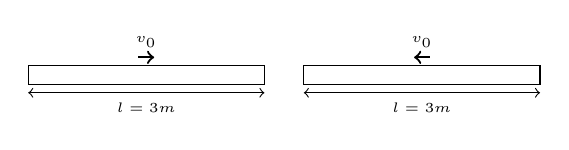
\begin{tikzpicture}
        \draw (0,0) rectangle (3,0.25);
        \draw[<->] (0,-0.1) -- (3,-0.1) node [midway, below] {\tiny $l=3m$};
        \draw[->,thick] (1.4,0.35) -- (1.6,0.35) node [midway, above] {\tiny $v_0$};
        \draw[<->] (3.5,-0.1) -- (6.5,-0.1) node [midway, below] {\tiny $l=3m$};
        \draw[<-,thick] (4.9,0.35) -- (5.1,0.35) node [midway, above] {\tiny $v_0$};
    
        \draw (3.5,0) rectangle (6.5,0.25);
      \end{tikzpicture}
    \end{column}
    \begin{footnotesize}
      \begin{column}{0.49\textwidth}
        $v_0=2.53 \: m/s $; $E= 2\times 10^{11} \: Pa$; $\rho = 7800 \: kg/m^{3}$
      \end{column}
    \end{footnotesize}
  \end{columns}
  \pause
  \centering
  \begin{tikzpicture}[scale=.6]
\begin{groupplot}[group style={group size=2 by 1,
ylabels at=edge left, yticklabels at=edge left,horizontal sep=2.ex,
vertical sep=2ex,xticklabels at=edge bottom,xlabels at=edge bottom},
ymajorgrids=true,xmajorgrids=true,enlargelimits=0,xmin=0.,xmax=6.,xlabel=$x (m)$,
axis on top,scale only axis,width=0.45\linewidth
]
\nextgroupplot[ylabel=$v (m/s)$,ymin=-2.785033259480085,ymax=2.785033259480085,title={(a) time $t = 1.21\times 10^{-4} $ s.},]
\addplot[Red,dashed,mark=none,very thick,mark size=3pt,mark repeat=2] coordinates{(0.0,2.5318484177091665) (0.12244897959183673,2.5318484177091665) (0.24489795918367346,2.531848417709166) (0.36734693877551017,2.531848417709166) (0.4897959183673469,2.5318484177091656) (0.6122448979591837,2.5318484177091665) (0.7346938775510203,2.531848417709167) (0.8571428571428571,2.5318484177091665) (0.9795918367346939,2.5318484177091665) (1.1020408163265305,2.5318484177091665) (1.2244897959183674,2.5318484177091665) (1.346938775510204,2.5318484177091665) (1.4693877551020407,2.5318484177091665) (1.5918367346938775,2.5318484177091665) (1.7142857142857142,2.5318484177091665) (1.836734693877551,2.531684227710154) (1.9591836734693877,2.528883339491711) (2.0816326530612246,2.5069977784469075) (2.204081632653061,2.405451093175476) (2.326530612244898,2.0843630627542513) (2.4489795918367347,1.4571958994685654) (2.571428571428571,0.3681332942558399) (2.693877551020408,0.03859430800310576) (2.816326530612245,-0.9060776804312415) (2.9387755102040813,0.15497604259705183) (3.061224489795918,-0.15497604259704956) (3.183673469387755,0.9060776804312402) (3.306122448979592,-0.038594308003106204) (3.4285714285714284,-0.3681332942558391) (3.5510204081632653,-1.4571958994685674) (3.673469387755102,-2.084363062754252) (3.7959183673469385,-2.4054510931754756) (3.9183673469387754,-2.506997778446907) (4.040816326530612,-2.5288833394917107) (4.163265306122449,-2.531684227710154) (4.285714285714286,-2.5318484177091665) (4.408163265306122,-2.5318484177091665) (4.530612244897959,-2.5318484177091665) (4.653061224489796,-2.5318484177091665) (4.775510204081632,-2.5318484177091665) (4.8979591836734695,-2.5318484177091665) (5.020408163265306,-2.5318484177091665) (5.142857142857142,-2.5318484177091665) (5.26530612244898,-2.5318484177091665) (5.387755102040816,-2.5318484177091665) (5.5102040816326525,-2.5318484177091665) (5.63265306122449,-2.5318484177091665) (5.755102040816326,-2.5318484177091665) (5.877551020408163,-2.5318484177091665) (6.0,-2.5318484177091665) };
\addplot[Orange,densely dotted,mark=none,very thick,mark size=3pt,mark repeat=2] coordinates{(0.0,2.5318484177091665) (0.06060606060606061,2.5318484177091665) (0.12121212121212122,2.5318484177091665) (0.18181818181818182,2.5318484177091665) (0.24242424242424243,2.5318484177091665) (0.30303030303030304,2.5318484177091665) (0.36363636363636365,2.5318484177091665) (0.42424242424242425,2.5318484177091665) (0.48484848484848486,2.5318484177091665) (0.5454545454545454,2.5318484177091665) (0.6060606060606061,2.5318484177091665) (0.6666666666666667,2.531848417709167) (0.7272727272727273,2.531848417709167) (0.7878787878787878,2.5318484177091665) (0.8484848484848485,2.5318484177091665) (0.9090909090909092,2.5318484177091674) (0.9696969696969697,2.5318484177091665) (1.0303030303030303,2.5318484177091665) (1.0909090909090908,2.5318484177091656) (1.1515151515151516,2.5318484177091665) (1.2121212121212122,2.5318484177091665) (1.2727272727272727,2.5318484177091665) (1.3333333333333335,2.5318484177091656) (1.393939393939394,2.531848417709166) (1.4545454545454546,2.5318484177091665) (1.5151515151515151,2.5318484177091656) (1.5757575757575757,2.5318484177091665) (1.6363636363636365,2.531848417709167) (1.696969696969697,2.5318484177091665) (1.7575757575757576,2.5318484177091665) (1.8181818181818183,2.5318020034751854) (1.878787878787879,2.5317091750072236) (1.9393939393939394,2.5307501424302727) (2.0,2.5289249057443333) (2.0606060606060606,2.5201129167796545) (2.121212121212121,2.504314175536237) (2.1818181818181817,2.4573457248537327) (2.2424242424242427,2.379207564732142) (2.303030303030303,2.2185258725100665) (2.3636363636363638,1.975300648187503) (2.4242424242424243,1.625621223269172) (2.484848484848485,1.1694875977550743) (2.5454545454545454,0.6521580355962723) (2.606060606060606,0.07363253679276927) (2.666666666666667,-0.20959340058418097) (2.7272727272727275,-0.1975197765345734) (2.787878787878788,-0.4134073094303823) (2.8484848484848486,-0.8572559992716083) (2.909090909090909,-0.17642315371687442) (2.9696969696969697,1.6290912272338196) (3.0303030303030303,-1.6290912272338194) (3.090909090909091,0.17642315371686795) (3.1515151515151514,0.8572559992716065) (3.2121212121212124,0.41340730943038484) (3.272727272727273,0.19751977653457933) (3.3333333333333335,0.20959340058418124) (3.393939393939394,-0.07363253679276877) (3.4545454545454546,-0.6521580355962722) (3.515151515151515,-1.1694875977550738) (3.5757575757575757,-1.6256212232691716) (3.6363636363636367,-1.9753006481875028) (3.6969696969696972,-2.2185258725100656) (3.757575757575758,-2.3792075647321425) (3.8181818181818183,-2.457345724853733) (3.878787878787879,-2.5043141755362366) (3.9393939393939394,-2.520112916779654) (4.0,-2.528924905744333) (4.0606060606060606,-2.5307501424302727) (4.121212121212121,-2.5317091750072236) (4.181818181818182,-2.531802003475186) (4.242424242424242,-2.5318484177091665) (4.303030303030303,-2.5318484177091665) (4.363636363636363,-2.5318484177091665) (4.424242424242425,-2.5318484177091665) (4.484848484848485,-2.5318484177091665) (4.545454545454546,-2.5318484177091665) (4.606060606060606,-2.5318484177091665) (4.666666666666667,-2.5318484177091665) (4.7272727272727275,-2.5318484177091665) (4.787878787878788,-2.5318484177091665) (4.848484848484849,-2.5318484177091665) (4.909090909090909,-2.5318484177091665) (4.96969696969697,-2.5318484177091665) (5.03030303030303,-2.5318484177091665) (5.090909090909091,-2.5318484177091665) (5.151515151515151,-2.5318484177091665) (5.212121212121212,-2.5318484177091665) (5.2727272727272725,-2.5318484177091665) (5.333333333333334,-2.5318484177091665) (5.3939393939393945,-2.5318484177091665) (5.454545454545455,-2.5318484177091665) (5.515151515151516,-2.5318484177091665) (5.575757575757576,-2.5318484177091665) (5.636363636363637,-2.5318484177091665) (5.696969696969697,-2.5318484177091665) (5.757575757575758,-2.5318484177091665) (5.818181818181818,-2.5318484177091665) (5.878787878787879,-2.5318484177091665) (5.9393939393939394,-2.5318484177091665) (6.0,-2.5318484177091665) };
\addplot[Duck,solid,mark=*,thick,mark size=2pt,mark repeat=2] coordinates{(0.0,2.5318484177091665) (0.06060606060606061,2.5318484177091665) (0.12121212121212122,2.5318484177091665) (0.18181818181818182,2.5318484177091665) (0.24242424242424243,2.531848417709166) (0.30303030303030304,2.531848417709166) (0.36363636363636365,2.531848417709166) (0.42424242424242425,2.531848417709166) (0.48484848484848486,2.531848417709166) (0.5454545454545454,2.531848417709166) (0.6060606060606061,2.531848417709166) (0.6666666666666667,2.531848417709166) (0.7272727272727273,2.531848417709166) (0.7878787878787878,2.531848417709166) (0.8484848484848485,2.531848417709166) (0.9090909090909092,2.531848417709166) (0.9696969696969697,2.531848417709166) (1.0303030303030303,2.5318484177091656) (1.0909090909090908,2.531848417709166) (1.1515151515151516,2.531848417709166) (1.2121212121212122,2.5318484177091665) (1.2727272727272727,2.5318484177091665) (1.3333333333333335,2.5318484177091665) (1.393939393939394,2.5318484177091665) (1.4545454545454546,2.5318484177091665) (1.5151515151515151,2.5318484177091665) (1.5757575757575757,2.5318484177091665) (1.6363636363636365,2.5318484177091665) (1.696969696969697,2.5318484177091665) (1.7575757575757576,2.5318484177091665) (1.8181818181818183,2.5314767282665054) (1.878787878787879,2.530733349381183) (1.9393939393939394,2.5251504222424406) (2.0,2.5147279468502757) (2.0606060606060606,2.4791562919092076) (2.121212121212121,2.418435457419236) (2.1818181818181817,2.293184610622088) (2.2424242424242427,2.1034037515177637) (2.303030303030303,1.8369856040367076) (2.3636363636363638,1.4939301681789166) (2.4242424242424243,1.1415549355096852) (2.484848484848485,0.7798599060290146) (2.5454545454545454,0.49089965505724753) (2.606060606060606,0.2746741825943853) (2.666666666666667,0.13130830787569914) (2.7272727272727275,0.060802030901189776) (2.787878787878788,0.019549701006694658) (2.8484848484848486,0.007551318192214021) (2.909090909090909,0.0011640950887300435) (2.9696969696969697,0.00038803169624276515) (3.0303030303030303,-0.0003880316962443448) (3.090909090909091,-0.0011640950887312836) (3.1515151515151514,-0.007551318192214904) (3.2121212121212124,-0.019549701006695293) (3.272727272727273,-0.0608020309011897) (3.3333333333333335,-0.13130830787569833) (3.393939393939394,-0.2746741825943841) (3.4545454545454546,-0.49089965505724675) (3.515151515151515,-0.7798599060290139) (3.5757575757575757,-1.141554935509685) (3.6363636363636367,-1.4939301681789163) (3.6969696969696972,-1.8369856040367067) (3.757575757575758,-2.1034037515177646) (3.8181818181818183,-2.2931846106220877) (3.878787878787879,-2.418435457419236) (3.9393939393939394,-2.479156291909208) (4.0,-2.514727946850276) (4.0606060606060606,-2.52515042224244) (4.121212121212121,-2.5307333493811837) (4.181818181818182,-2.5314767282665054) (4.242424242424242,-2.5318484177091665) (4.303030303030303,-2.5318484177091665) (4.363636363636363,-2.5318484177091665) (4.424242424242425,-2.5318484177091665) (4.484848484848485,-2.5318484177091665) (4.545454545454546,-2.5318484177091665) (4.606060606060606,-2.5318484177091665) (4.666666666666667,-2.5318484177091665) (4.7272727272727275,-2.5318484177091665) (4.787878787878788,-2.5318484177091665) (4.848484848484849,-2.5318484177091665) (4.909090909090909,-2.5318484177091665) (4.96969696969697,-2.5318484177091665) (5.03030303030303,-2.5318484177091665) (5.090909090909091,-2.5318484177091665) (5.151515151515151,-2.5318484177091665) (5.212121212121212,-2.5318484177091665) (5.2727272727272725,-2.5318484177091665) (5.333333333333334,-2.5318484177091665) (5.3939393939393945,-2.5318484177091665) (5.454545454545455,-2.5318484177091665) (5.515151515151516,-2.5318484177091665) (5.575757575757576,-2.5318484177091665) (5.636363636363637,-2.5318484177091665) (5.696969696969697,-2.5318484177091665) (5.757575757575758,-2.5318484177091665) (5.818181818181818,-2.5318484177091665) (5.878787878787879,-2.5318484177091665) (5.9393939393939394,-2.5318484177091665) (6.0,-2.5318484177091665) };
\addplot[Blue,solid,mark=none,very thick,mark size=3pt,mark repeat=2] coordinates{(0.0,2.531848417709167) (0.12244897959183673,2.5318484177091656) (0.24489795918367346,2.531848417709166) (0.36734693877551017,2.5318484177091665) (0.4897959183673469,2.531848417709166) (0.6122448979591837,2.531848417709166) (0.7346938775510203,2.531848417709166) (0.8571428571428571,2.531848417709166) (0.9795918367346939,2.531848417709166) (1.1020408163265305,2.531848417709166) (1.2244897959183674,2.5318484177091656) (1.346938775510204,2.531848417709166) (1.4693877551020407,2.531848417709166) (1.5918367346938775,2.5318484177091665) (1.7142857142857142,2.531848417709166) (1.836734693877551,2.531848417709167) (1.9591836734693877,2.5318484177091665) (2.0816326530612246,2.5318484177091665) (2.204081632653061,2.5318484177091665) (2.326530612244898,2.5318484177091665) (2.4489795918367347,0.0) (2.571428571428571,-1.131824441720173e-15) (2.693877551020408,3.772748139067242e-16) (2.816326530612245,-3.944304526105059e-31) (2.9387755102040813,7.545496278134482e-16) (3.061224489795918,-1.131824441720173e-15) (3.183673469387755,3.772748139067241e-16) (3.306122448979592,3.772748139067244e-16) (3.4285714285714284,7.545496278134485e-16) (3.5510204081632653,2.220446049250313e-16) (3.673469387755102,-2.5318484177091665) (3.7959183673469385,-2.531848417709166) (3.9183673469387754,-2.531848417709166) (4.040816326530612,-2.531848417709167) (4.163265306122449,-2.531848417709166) (4.285714285714286,-2.5318484177091656) (4.408163265306122,-2.531848417709167) (4.530612244897959,-2.5318484177091665) (4.653061224489796,-2.531848417709166) (4.775510204081632,-2.531848417709167) (4.8979591836734695,-2.5318484177091665) (5.020408163265306,-2.531848417709167) (5.142857142857142,-2.531848417709167) (5.26530612244898,-2.531848417709167) (5.387755102040816,-2.531848417709167) (5.5102040816326525,-2.531848417709167) (5.63265306122449,-2.5318484177091665) (5.755102040816326,-2.531848417709166) (5.877551020408163,-2.531848417709167) (6.0,-2.5318484177091665) };
\addplot[Purple,solid,mark=+,very thick,mark size=3pt,mark repeat=2] coordinates{(0.0,2.531848417709166) (0.06060606060606061,2.531848417709166) (0.12121212121212122,2.531848417709166) (0.18181818181818182,2.531848417709166) (0.24242424242424243,2.5318484177091656) (0.30303030303030304,2.5318484177091656) (0.36363636363636365,2.5318484177091656) (0.42424242424242425,2.5318484177091656) (0.48484848484848486,2.5318484177091656) (0.5454545454545454,2.531848417709165) (0.6060606060606061,2.531848417709165) (0.6666666666666667,2.531848417709165) (0.7272727272727273,2.531848417709165) (0.7878787878787878,2.531848417709165) (0.8484848484848485,2.531848417709165) (0.9090909090909092,2.5318484177091647) (0.9696969696969697,2.5318484177091647) (1.0303030303030303,2.5318484177091647) (1.0909090909090908,2.5318484177091647) (1.1515151515151516,2.531848417709165) (1.2121212121212122,2.531848417709165) (1.2727272727272727,2.531848417709165) (1.3333333333333335,2.531848417709165) (1.393939393939394,2.531848417709165) (1.4545454545454546,2.531848417709165) (1.5151515151515151,2.5318484177091656) (1.5757575757575757,2.5318484177091656) (1.6363636363636365,2.531848417709166) (1.696969696969697,2.531848417709166) (1.7575757575757576,2.531848417709166) (1.8181818181818183,2.5317555939571394) (1.878787878787879,2.5315699464530863) (1.9393939393939394,2.529300921403548) (2.0,2.5251960488139282) (2.0606060606060606,2.502983668745643) (2.121212121212121,2.4672568379656363) (2.1818181818181817,2.3558296271378385) (2.2424242424242427,2.199909152499134) (2.303030303030303,1.8955358394101423) (2.3636363636363638,1.5350380403392951) (2.4242424242424243,1.0913569359704094) (2.484848484848485,0.6616953448225573) (2.5454545454545454,0.35041226238060424) (2.606060606060606,0.11398111608931762) (2.666666666666667,0.037623711953108305) (2.7272727272727275,-0.006618739561512254) (2.787878787878788,-0.0024042733543885486) (2.8484848484848486,-0.0017885136987410197) (2.909090909090909,-0.0001900946309221662) (2.9696969696969697,4.075039583706578e-05) (3.0303030303030303,-4.075039583690026e-05) (3.090909090909091,0.000190094630922048) (3.1515151515151514,0.001788513698741276) (3.2121212121212124,0.0024042733543890842) (3.272727272727273,0.006618739561513227) (3.3333333333333335,-0.03762371195310714) (3.393939393939394,-0.11398111608931744) (3.4545454545454546,-0.35041226238060363) (3.515151515151515,-0.6616953448225579) (3.5757575757575757,-1.09135693597041) (3.6363636363636367,-1.535038040339297) (3.6969696969696972,-1.8955358394101425) (3.757575757575758,-2.199909152499135) (3.8181818181818183,-2.3558296271378385) (3.878787878787879,-2.4672568379656363) (3.9393939393939394,-2.502983668745643) (4.0,-2.5251960488139282) (4.0606060606060606,-2.5293009214035473) (4.121212121212121,-2.5315699464530863) (4.181818181818182,-2.5317555939571394) (4.242424242424242,-2.531848417709166) (4.303030303030303,-2.531848417709166) (4.363636363636363,-2.531848417709166) (4.424242424242425,-2.531848417709166) (4.484848484848485,-2.531848417709166) (4.545454545454546,-2.531848417709166) (4.606060606060606,-2.531848417709166) (4.666666666666667,-2.531848417709166) (4.7272727272727275,-2.531848417709166) (4.787878787878788,-2.531848417709166) (4.848484848484849,-2.531848417709166) (4.909090909090909,-2.531848417709166) (4.96969696969697,-2.531848417709166) (5.03030303030303,-2.531848417709166) (5.090909090909091,-2.531848417709166) (5.151515151515151,-2.531848417709166) (5.212121212121212,-2.531848417709166) (5.2727272727272725,-2.531848417709166) (5.333333333333334,-2.531848417709166) (5.3939393939393945,-2.531848417709166) (5.454545454545455,-2.531848417709166) (5.515151515151516,-2.531848417709166) (5.575757575757576,-2.531848417709166) (5.636363636363637,-2.531848417709166) (5.696969696969697,-2.531848417709166) (5.757575757575758,-2.531848417709166) (5.818181818181818,-2.531848417709166) (5.878787878787879,-2.531848417709166) (5.9393939393939394,-2.531848417709166) (6.0,-2.5318484177091665) };
\addplot[Green,only marks,mark=x,thick,mark size=3pt,mark repeat=2] coordinates{(0.0,2.531848417709166) (0.06060606060606061,2.531848417709166) (0.12121212121212122,2.531848417709166) (0.18181818181818182,2.531848417709166) (0.24242424242424243,2.5318484177091665) (0.30303030303030304,2.5318484177091665) (0.36363636363636365,2.5318484177091656) (0.42424242424242425,2.5318484177091656) (0.48484848484848486,2.5318484177091665) (0.5454545454545454,2.5318484177091665) (0.6060606060606061,2.531848417709165) (0.6666666666666667,2.5318484177091656) (0.7272727272727273,2.531848417709166) (0.7878787878787878,2.531848417709166) (0.8484848484848485,2.5318484177091656) (0.9090909090909092,2.5318484177091656) (0.9696969696969697,2.5318484177091665) (1.0303030303030303,2.5318484177091665) (1.0909090909090908,2.5318484177091647) (1.1515151515151516,2.531848417709165) (1.2121212121212122,2.531848417709166) (1.2727272727272727,2.531848417709166) (1.3333333333333335,2.5318484177091647) (1.393939393939394,2.5318484177091647) (1.4545454545454546,2.5318484177091665) (1.5151515151515151,2.5318484177091665) (1.5757575757575757,2.531848417709166) (1.6363636363636365,2.531848417709166) (1.696969696969697,2.531848417709166) (1.7575757575757576,2.531848417709166) (1.8181818181818183,2.531848417709166) (1.878787878787879,2.531848417709166) (1.9393939393939394,2.531848417709166) (2.0,2.531848417709166) (2.0606060606060606,2.5318484177091656) (2.121212121212121,2.531848417709166) (2.1818181818181817,2.5318484177091665) (2.2424242424242427,2.531848417709166) (2.303030303030303,2.5318484177091665) (2.3636363636363638,2.5318484177091665) (2.4242424242424243,7.771561172376108e-16) (2.484848484848485,-2.1094237467877935e-15) (2.5454545454545454,-2.4980018054065835e-16) (2.606060606060606,-1.0824674490095235e-15) (2.666666666666667,8.52730145933733e-16) (2.7272727272727275,8.332007357698796e-16) (2.787878787878788,-6.636926385046085e-16) (2.8484848484848486,-6.685749910455732e-16) (2.909090909090909,-9.666384036373804e-17) (2.9696969696969697,2.734954664404533e-16) (3.0303030303030303,-9.789796087117351e-17) (3.090909090909091,9.860763805712963e-16) (3.1515151515151514,-5.850647289005321e-16) (3.2121212121212124,-3.585610702627896e-17) (3.272727272727273,8.518216860046792e-17) (3.3333333333333335,-1.2838500279050285e-16) (3.393939393939394,1.7783669840585248e-16) (3.4545454545454546,8.942088536749598e-17) (3.515151515151515,-9.992007221626425e-16) (3.5757575757575757,2.331468351712824e-15) (3.6363636363636367,-2.531848417709166) (3.6969696969696972,-2.5318484177091665) (3.757575757575758,-2.531848417709166) (3.8181818181818183,-2.5318484177091665) (3.878787878787879,-2.531848417709166) (3.9393939393939394,-2.5318484177091665) (4.0,-2.531848417709166) (4.0606060606060606,-2.531848417709166) (4.121212121212121,-2.531848417709166) (4.181818181818182,-2.531848417709166) (4.242424242424242,-2.5318484177091665) (4.303030303030303,-2.531848417709167) (4.363636363636363,-2.531848417709165) (4.424242424242425,-2.531848417709165) (4.484848484848485,-2.5318484177091665) (4.545454545454546,-2.5318484177091665) (4.606060606060606,-2.5318484177091665) (4.666666666666667,-2.5318484177091665) (4.7272727272727275,-2.5318484177091656) (4.787878787878788,-2.531848417709166) (4.848484848484849,-2.531848417709166) (4.909090909090909,-2.5318484177091665) (4.96969696969697,-2.531848417709166) (5.03030303030303,-2.5318484177091665) (5.090909090909091,-2.531848417709166) (5.151515151515151,-2.5318484177091665) (5.212121212121212,-2.531848417709166) (5.2727272727272725,-2.5318484177091665) (5.333333333333334,-2.531848417709166) (5.3939393939393945,-2.5318484177091665) (5.454545454545455,-2.531848417709166) (5.515151515151516,-2.5318484177091665) (5.575757575757576,-2.531848417709166) (5.636363636363637,-2.5318484177091665) (5.696969696969697,-2.531848417709166) (5.757575757575758,-2.5318484177091665) (5.818181818181818,-2.531848417709166) (5.878787878787879,-2.5318484177091665) (5.9393939393939394,-2.5318484177091665) (6.0,-2.5318484177091665) };
\addplot[black,solid,mark=pentagone*,thin,mark size=3pt,mark repeat=2] coordinates{(0.0,2.5318484177091665) (0.12244897959183673,2.5318484177091665) (0.24489795918367346,2.5318484177091665) (0.36734693877551017,2.5318484177091665) (0.4897959183673469,2.5318484177091665) (0.6122448979591837,2.5318484177091665) (0.7346938775510203,2.5318484177091665) (0.8571428571428571,2.5318484177091665) (0.9795918367346939,2.5318484177091665) (1.1020408163265305,2.5318484177091665) (1.2244897959183674,2.5318484177091665) (1.346938775510204,2.5318484177091665) (1.4693877551020407,2.5318484177091665) (1.5918367346938775,2.5318484177091665) (1.7142857142857142,2.5318484177091665) (1.836734693877551,2.5318484177091665) (1.9591836734693877,2.5318484177091665) (2.0816326530612246,2.5318484177091665) (2.204081632653061,2.5318484177091665) (2.326530612244898,2.5318484177091665) (2.4489795918367347,0.0) (2.571428571428571,0.0) (2.693877551020408,0.0) (2.816326530612245,0.0) (2.9387755102040813,0.0) (3.061224489795918,-0.0) (3.183673469387755,-0.0) (3.306122448979592,-0.0) (3.4285714285714284,-0.0) (3.5510204081632653,-0.0) (3.673469387755102,-2.5318484177091665) (3.7959183673469385,-2.5318484177091665) (3.9183673469387754,-2.5318484177091665) (4.040816326530612,-2.5318484177091665) (4.163265306122449,-2.5318484177091665) (4.285714285714286,-2.5318484177091665) (4.408163265306122,-2.5318484177091665) (4.530612244897959,-2.5318484177091665) (4.653061224489796,-2.5318484177091665) (4.775510204081632,-2.5318484177091665) (4.8979591836734695,-2.5318484177091665) (5.020408163265306,-2.5318484177091665) (5.142857142857142,-2.5318484177091665) (5.26530612244898,-2.5318484177091665) (5.387755102040816,-2.5318484177091665) (5.5102040816326525,-2.5318484177091665) (5.63265306122449,-2.5318484177091665) (5.755102040816326,-2.5318484177091665) (5.877551020408163,-2.5318484177091665) (6.0,-2.5318484177091665) };
\nextgroupplot[legend style={at={($(0.7,-0.35)+(5.9cm,8cm)$)},legend columns=1},ymin=-2.785033259480085,ymax=2.785033259480085,title={(b) time $t = 4.84\times 10^{-4} $ s.}]
\addplot[Red,dashed,mark=none,very thick,mark size=3pt,mark repeat=2] coordinates{(0.0,2.5318484177091665) (0.12244897959183673,2.531848417709167) (0.24489795918367346,2.531848417709166) (0.36734693877551017,2.531848417709166) (0.4897959183673469,2.531848417709165) (0.6122448979591837,2.5318483984539664) (0.7346938775510203,2.5318477659475827) (0.8571428571428571,2.5318378383698152) (0.9795918367346939,2.531738909821285) (1.1020408163265305,2.5310376550966116) (1.2244897959183674,2.5272846058424623) (1.346938775510204,2.511582995381506) (1.4693877551020407,2.4591766365643473) (1.5918367346938775,2.3181168751417087) (1.7142857142857142,2.0117581239436237) (1.836734693877551,1.477297258708373) (1.9591836734693877,0.7554822113442998) (2.0816326530612246,0.010684165656105471) (2.204081632653061,-0.39396688397347013) (2.326530612244898,-0.5189112540071943) (2.4489795918367347,-0.020711514080181737) (2.571428571428571,-0.04925338946186149) (2.693877551020408,0.3772292528240989) (2.816326530612245,-0.28486682427919574) (2.9387755102040813,0.279534610825791) (3.061224489795918,-0.2795346108257906) (3.183673469387755,0.2848668242791922) (3.306122448979592,-0.37722925282409936) (3.4285714285714284,0.04925338946185971) (3.5510204081632653,0.020711514080185872) (3.673469387755102,0.518911254007197) (3.7959183673469385,0.3939668839734717) (3.9183673469387754,-0.010684165656106692) (4.040816326530612,-0.7554822113442974) (4.163265306122449,-1.477297258708377) (4.285714285714286,-2.011758123943624) (4.408163265306122,-2.3181168751417087) (4.530612244897959,-2.459176636564347) (4.653061224489796,-2.511582995381506) (4.775510204081632,-2.5272846058424627) (4.8979591836734695,-2.5310376550966107) (5.020408163265306,-2.531738909821284) (5.142857142857142,-2.531837838369815) (5.26530612244898,-2.5318477659475827) (5.387755102040816,-2.5318483984539664) (5.5102040816326525,-2.5318484177091665) (5.63265306122449,-2.5318484177091665) (5.755102040816326,-2.5318484177091665) (5.877551020408163,-2.5318484177091665) (6.0,-2.5318484177091665) };
\addplot[Orange,densely dotted,mark=none,very thick,mark size=3pt,mark repeat=2] coordinates{(0.0,2.5318484177091665) (0.06060606060606061,2.5318484177091665) (0.12121212121212122,2.5318484177091665) (0.18181818181818182,2.5318484177091665) (0.24242424242424243,2.5318484177091665) (0.30303030303030304,2.5318484177091665) (0.36363636363636365,2.5318484177091665) (0.42424242424242425,2.5318484177091665) (0.48484848484848486,2.5318484177091665) (0.5454545454545454,2.5318484177091665) (0.6060606060606061,2.5318484151568073) (0.6666666666666667,2.531848410052089) (0.7272727272727273,2.5318483062561463) (0.7878787878787878,2.5318481037689806) (0.8484848484848485,2.5318461134959485) (0.9090909090909092,2.5318423354370503) (0.9696969696969697,2.531818445166049) (1.0303030303030303,2.531774442682947) (1.0909090909090908,2.531573501160723) (1.1515151515151516,2.531215620599377) (1.2121212121212122,2.529959996602834) (1.2727272727272727,2.5278066291710957) (1.3333333333333335,2.5217797302083578) (1.393939393939394,2.5118792997146255) (1.4545454545454546,2.489236665383997) (1.5151515151515151,2.4538518272164733) (1.5757575757575757,2.3867144217459435) (1.6363636363636365,2.2878244489724064) (1.696969696969697,2.1309266174919825) (1.7575757575757576,1.9160209273046755) (1.8181818181818183,1.6307338302347996) (1.878787878787879,1.2750653262823581) (1.9393939393939394,0.8846124649872573) (2.0,0.45937524634950305) (2.0606060606060606,0.08727763903668462) (2.121212121212121,-0.23168035695119626) (2.1818181818181817,-0.4175483709794803) (2.2424242424242427,-0.4703264030481671) (2.303030303030303,-0.41875637304195895) (2.3636363636363638,-0.26283828096085887) (2.4242424242424243,-0.0954921221874162) (2.484848484848485,0.08328210327836835) (2.5454545454545454,0.14407234790709328) (2.606060606060606,0.08687861169875953) (2.666666666666667,0.11137418504956392) (2.7272727272727275,0.21755906795950974) (2.787878787878788,-0.02803136011717798) (2.8484848484848486,-0.6253970991805003) (2.909090909090909,-0.06009787210682943) (2.9696969696969697,1.6678663211038354) (3.0303030303030303,-1.6678663211038323) (3.090909090909091,0.06009787210682655) (3.1515151515151514,0.6253970991805009) (3.2121212121212124,0.028031360117178453) (3.272727272727273,-0.21755906795950636) (3.3333333333333335,-0.1113741850495652) (3.393939393939394,-0.08687861169876046) (3.4545454545454546,-0.14407234790709447) (3.515151515151515,-0.08328210327836953) (3.5757575757575757,0.09549212218741482) (3.6363636363636367,0.26283828096085826) (3.6969696969696972,0.4187563730419601) (3.757575757575758,0.47032640304816764) (3.8181818181818183,0.4175483709794797) (3.878787878787879,0.2316803569511961) (3.9393939393939394,-0.0872776390366839) (4.0,-0.4593752463495025) (4.0606060606060606,-0.8846124649872572) (4.121212121212121,-1.275065326282357) (4.181818181818182,-1.6307338302348002) (4.242424242424242,-1.916020927304675) (4.303030303030303,-2.130926617491981) (4.363636363636363,-2.2878244489724056) (4.424242424242425,-2.3867144217459453) (4.484848484848485,-2.4538518272164747) (4.545454545454546,-2.4892366653839972) (4.606060606060606,-2.5118792997146255) (4.666666666666667,-2.5217797302083578) (4.7272727272727275,-2.5278066291710943) (4.787878787878788,-2.5299599966028334) (4.848484848484849,-2.5312156205993763) (4.909090909090909,-2.5315735011607234) (4.96969696969697,-2.5317744426829467) (5.03030303030303,-2.5318184451660493) (5.090909090909091,-2.53184233543705) (5.151515151515151,-2.531846113495948) (5.212121212121212,-2.53184810376898) (5.2727272727272725,-2.5318483062561463) (5.333333333333334,-2.531848410052089) (5.3939393939393945,-2.5318484151568073) (5.454545454545455,-2.5318484177091665) (5.515151515151516,-2.5318484177091665) (5.575757575757576,-2.5318484177091665) (5.636363636363637,-2.5318484177091665) (5.696969696969697,-2.5318484177091665) (5.757575757575758,-2.5318484177091665) (5.818181818181818,-2.5318484177091665) (5.878787878787879,-2.5318484177091665) (5.9393939393939394,-2.5318484177091665) (6.0,-2.5318484177091665) };
\addplot[Duck,solid,mark=*,thick,mark size=2pt,mark repeat=2] coordinates{(0.0,2.531848417709166) (0.06060606060606061,2.531848417709166) (0.12121212121212122,2.531848417709166) (0.18181818181818182,2.531848417709166) (0.24242424242424243,2.531848417709166) (0.30303030303030304,2.531848417709166) (0.36363636363636365,2.531848417709166) (0.42424242424242425,2.531848417709166) (0.48484848484848486,2.531848417709166) (0.5454545454545454,2.531848417709166) (0.6060606060606061,2.531848322218527) (0.6666666666666667,2.5318481312372487) (0.7272727272727273,2.5318451768738073) (0.7878787878787878,2.531839459128202) (0.8484848484848485,2.5317972741399446) (0.9090909090909092,2.531718621909035) (0.9696969696969697,2.531349985135261) (1.0303030303030303,2.530691363818622) (1.0909090909090908,2.528487041474035) (1.1515151515151516,2.5247370181015003) (1.2121212121212122,2.5151819070173778) (1.2727272727272727,2.499821708221668) (1.3333333333333335,2.4687849694057875) (1.393939393939394,2.4220716905697377) (1.4545454545454546,2.3450324107320544) (1.5151515151515151,2.2376671298927375) (1.5757575757575757,2.0899010681921935) (1.6363636363636365,1.9017342256304213) (1.696969696969697,1.6815563242811924) (1.7575757575757576,1.4293673641445055) (1.8181818181818183,1.1742121642120082) (1.878787878787879,0.9160907244837013) (1.9393939393939394,0.6865647991400854) (2.0,0.4856343881811611) (2.0606060606060606,0.32603252055315013) (2.121212121212121,0.2077591962560531) (2.1818181818181817,0.12249073841136798) (2.2424242424242427,0.0702271470190948) (2.303030303030303,0.03551770611448978) (2.3636363636363638,0.01836241569755198) (2.4242424242424243,0.007729710698309033) (2.484848484848485,0.003619591116760991) (2.5454545454545454,0.0012158346463164134) (2.606060606060606,0.0005184412869753138) (2.666666666666667,0.00013011416411164403) (2.7272727272727275,5.085327772540678e-05) (2.787878787878788,8.496748645186023e-06) (2.8484848484848486,3.0445768709820515e-06) (2.909090909090909,2.3886823801310813e-07) (2.9696969696969697,7.962274627921281e-08) (3.0303030303030303,-7.96227454470489e-08) (3.090909090909091,-2.388682371656764e-07) (3.1515151515151514,-3.044576870427015e-06) (3.2121212121212124,-8.496748645231104e-06) (3.272727272727273,-5.0853277725753164e-05) (3.3333333333333335,-0.00013011416411199333) (3.393939393939394,-0.0005184412869758035) (3.4545454545454546,-0.0012158346463171834) (3.515151515151515,-0.0036195911167619375) (3.5757575757575757,-0.007729710698310062) (3.6363636363636367,-0.018362415697552956) (3.6969696969696972,-0.0355177061144906) (3.757575757575758,-0.07022714701909577) (3.8181818181818183,-0.12249073841136837) (3.878787878787879,-0.2077591962560532) (3.9393939393939394,-0.32603252055315) (4.0,-0.4856343881811607) (4.0606060606060606,-0.686564799140085) (4.121212121212121,-0.9160907244837007) (4.181818181818182,-1.1742121642120076) (4.242424242424242,-1.4293673641445048) (4.303030303030303,-1.6815563242811915) (4.363636363636363,-1.9017342256304213) (4.424242424242425,-2.089901068192196) (4.484848484848485,-2.2376671298927384) (4.545454545454546,-2.3450324107320544) (4.606060606060606,-2.4220716905697377) (4.666666666666667,-2.468784969405788) (4.7272727272727275,-2.499821708221668) (4.787878787878788,-2.515181907017378) (4.848484848484849,-2.5247370181015008) (4.909090909090909,-2.528487041474035) (4.96969696969697,-2.530691363818622) (5.03030303030303,-2.531349985135261) (5.090909090909091,-2.5317186219090355) (5.151515151515151,-2.5317972741399446) (5.212121212121212,-2.5318394591282023) (5.2727272727272725,-2.5318451768738073) (5.333333333333334,-2.5318481312372496) (5.3939393939393945,-2.5318483222185275) (5.454545454545455,-2.5318484177091665) (5.515151515151516,-2.5318484177091665) (5.575757575757576,-2.5318484177091665) (5.636363636363637,-2.5318484177091665) (5.696969696969697,-2.5318484177091665) (5.757575757575758,-2.5318484177091665) (5.818181818181818,-2.5318484177091665) (5.878787878787879,-2.5318484177091665) (5.9393939393939394,-2.5318484177091665) (6.0,-2.5318484177091665) };
\addplot[Blue,solid,mark=none,very thick,mark size=3pt,mark repeat=2] coordinates{(0.0,2.5318484177091642) (0.12244897959183673,2.531848417709168) (0.24489795918367346,2.5318484177091647) (0.36734693877551017,2.531848417709165) (0.4897959183673469,2.531848417709166) (0.6122448979591837,2.531848417709166) (0.7346938775510203,2.531848417709166) (0.8571428571428571,2.531848417709167) (0.9795918367346939,2.531848417709166) (1.1020408163265305,2.531848417709166) (1.2244897959183674,2.5318484177091665) (1.346938775510204,2.531848417709166) (1.4693877551020407,2.531848417709166) (1.5918367346938775,2.531848417709166) (1.7142857142857142,2.531848417709166) (1.836734693877551,-6.661338147750939e-16) (1.9591836734693877,-2.485693488365377e-15) (2.0816326530612246,6.877352318701104e-16) (2.204081632653061,-5.9164567891575885e-31) (2.326530612244898,-3.7727481390672426e-16) (2.4489795918367347,3.944304526105059e-31) (2.571428571428571,1.1318244417201724e-15) (2.693877551020408,-5.9164567891575885e-31) (2.816326530612245,1.1318244417201723e-15) (2.9387755102040813,-3.944304526105059e-31) (3.061224489795918,-7.888609052210118e-31) (3.183673469387755,-3.772748139067248e-16) (3.306122448979592,2.2636488834403473e-15) (3.4285714285714284,-1.886374069533621e-15) (3.5510204081632653,2.1084186744586528e-15) (3.673469387755102,-9.981956498334958e-16) (3.7959183673469385,3.104604179633854e-16) (3.9183673469387754,-6.209208359267718e-16) (4.040816326530612,1.065010045776834e-15) (4.163265306122449,-1.5543122344752192e-15) (4.285714285714286,-2.531848417709166) (4.408163265306122,-2.531848417709167) (4.530612244897959,-2.5318484177091665) (4.653061224489796,-2.531848417709166) (4.775510204081632,-2.531848417709166) (4.8979591836734695,-2.531848417709166) (5.020408163265306,-2.5318484177091665) (5.142857142857142,-2.5318484177091665) (5.26530612244898,-2.531848417709166) (5.387755102040816,-2.5318484177091665) (5.5102040816326525,-2.531848417709167) (5.63265306122449,-2.531848417709167) (5.755102040816326,-2.531848417709167) (5.877551020408163,-2.531848417709167) (6.0,-2.531848417709168) };
\addplot[Purple,solid,mark=+,very thick,mark size=3pt,mark repeat=2] coordinates{(0.0,2.5318484177091625) (0.06060606060606061,2.5318484177091625) (0.12121212121212122,2.531848417709163) (0.18181818181818182,2.5318484177091634) (0.24242424242424243,2.5318484177091642) (0.30303030303030304,2.5318484177091642) (0.36363636363636365,2.531848417709164) (0.42424242424242425,2.531848417709164) (0.48484848484848486,2.531848417709164) (0.5454545454545454,2.531848417709164) (0.6060606060606061,2.5318484126044454) (0.6666666666666667,2.531848402395009) (0.7272727272727273,2.531848147159085) (0.7878787878787878,2.531847660509256) (0.8484848484848485,2.5318419112097796) (0.9090909090909092,2.5318314997267986) (0.9696969696969697,2.5317543577392794) (1.0303030303030303,2.531622226855984) (1.0909090909090908,2.5309352642773124) (1.1515151515151516,2.529827505784501) (1.2121212121212122,2.525544979109427) (1.2727272727272727,2.5190772040991836) (1.3333333333333335,2.49986453919368) (1.393939393939394,2.4728460487555486) (1.4545454545454546,2.4100439263485716) (1.5151515151515151,2.3283399292621993) (1.5757575757575757,2.178564100960003) (1.6363636363636365,1.999603107753429) (1.696969696969697,1.7412015276196833) (1.7575757575757576,1.4598954849283565) (1.8181818181818183,1.1436088819043788) (1.878787878787879,0.8326048422840917) (1.9393939393939394,0.5673667305700555) (2.0,0.3338637253193525) (2.0606060606060606,0.19081928650352253) (2.121212121212121,0.07885642245760108) (2.1818181818181817,0.035644258017509256) (2.2424242424242427,0.00543058051750829) (2.303030303030303,0.0012651237456281672) (2.3636363636363638,-0.0017052487095000686) (2.4242424242424243,-0.0006454300856452834) (2.484848484848485,-0.0002806339825737999) (2.5454545454545454,-6.316370952302816e-05) (2.606060606060606,1.1141267552461879e-05) (2.666666666666667,3.186617029754634e-06) (2.7272727272727275,2.224000786251848e-06) (2.787878787878788,2.458788272790853e-07) (2.8484848484848486,-4.858566390766534e-08) (2.909090909090909,-4.144118614765797e-09) (2.9696969696969697,-1.97507262108322e-09) (3.0303030303030303,1.9750719798293663e-09) (3.090909090909091,4.144118171518933e-09) (3.1515151515151514,4.8585664037513496e-08) (3.2121212121212124,-2.458788273706489e-07) (3.272727272727273,-2.2240007863010142e-06) (3.3333333333333335,-3.186617029443332e-06) (3.393939393939394,-1.114126755228617e-05) (3.4545454545454546,6.316370952276986e-05) (3.515151515151515,0.00028063398257326263) (3.5757575757575757,0.0006454300856452396) (3.6363636363636367,0.0017052487095003755) (3.6969696969696972,-0.001265123745628387) (3.757575757575758,-0.00543058051750882) (3.8181818181818183,-0.035644258017509936) (3.878787878787879,-0.0788564224576016) (3.9393939393939394,-0.19081928650352323) (4.0,-0.3338637253193546) (4.0606060606060606,-0.5673667305700569) (4.121212121212121,-0.8326048422840933) (4.181818181818182,-1.1436088819043795) (4.242424242424242,-1.4598954849283583) (4.303030303030303,-1.7412015276196846) (4.363636363636363,-1.9996031077534282) (4.424242424242425,-2.1785641009600054) (4.484848484848485,-2.328339929262201) (4.545454545454546,-2.410043926348574) (4.606060606060606,-2.4728460487555504) (4.666666666666667,-2.499864539193682) (4.7272727272727275,-2.519077204099186) (4.787878787878788,-2.525544979109429) (4.848484848484849,-2.5298275057845023) (4.909090909090909,-2.5309352642773137) (4.96969696969697,-2.531622226855986) (5.03030303030303,-2.5317543577392807) (5.090909090909091,-2.5318314997268) (5.151515151515151,-2.531841911209781) (5.212121212121212,-2.531847660509258) (5.2727272727272725,-2.5318481471590863) (5.333333333333334,-2.5318484023950107) (5.3939393939393945,-2.5318484126044476) (5.454545454545455,-2.531848417709166) (5.515151515151516,-2.531848417709166) (5.575757575757576,-2.531848417709166) (5.636363636363637,-2.531848417709166) (5.696969696969697,-2.531848417709166) (5.757575757575758,-2.531848417709166) (5.818181818181818,-2.531848417709166) (5.878787878787879,-2.531848417709166) (5.9393939393939394,-2.531848417709166) (6.0,-2.5318484177091665) };
\addplot[Green,only marks,mark=x,thick,mark size=3pt,mark repeat=2] coordinates{(0.0,2.531848417709165) (0.06060606060606061,2.5318484177091647) (0.12121212121212122,2.5318484177091647) (0.18181818181818182,2.531848417709165) (0.24242424242424243,2.5318484177091656) (0.30303030303030304,2.531848417709165) (0.36363636363636365,2.531848417709166) (0.42424242424242425,2.531848417709166) (0.48484848484848486,2.5318484177091642) (0.5454545454545454,2.531848417709164) (0.6060606060606061,2.531848417709166) (0.6666666666666667,2.531848417709166) (0.7272727272727273,2.5318484177091647) (0.7878787878787878,2.5318484177091647) (0.8484848484848485,2.5318484177091647) (0.9090909090909092,2.5318484177091647) (0.9696969696969697,2.531848417709166) (1.0303030303030303,2.531848417709166) (1.0909090909090908,2.531848417709166) (1.1515151515151516,2.531848417709166) (1.2121212121212122,2.5318484177091642) (1.2727272727272727,2.5318484177091642) (1.3333333333333335,2.5318484177091642) (1.393939393939394,2.5318484177091647) (1.4545454545454546,2.5318484177091647) (1.5151515151515151,2.5318484177091647) (1.5757575757575757,2.5318484177091647) (1.6363636363636365,2.5318484177091647) (1.696969696969697,2.5318484177091647) (1.7575757575757576,2.531848417709165) (1.8181818181818183,7.771561172376108e-16) (1.878787878787879,-2.1094237467877935e-15) (1.9393939393939394,-1.2428467441826863e-15) (2.0,-1.1544309311443312e-15) (2.0606060606060606,1.3696932073430366e-15) (2.121212121212121,1.2476189282507285e-15) (2.1818181818181817,-2.4419093580481207e-15) (2.2424242424242427,-2.085388408832536e-15) (2.303030303030303,1.2943623313739441e-17) (2.3636363636363638,-1.4657241520041104e-16) (2.4242424242424243,1.111119986946025e-15) (2.484848484848485,5.748108947575872e-16) (2.5454545454545454,-1.8234388364241851e-16) (2.606060606060606,-3.953741180943154e-16) (2.666666666666667,4.31804378727956e-16) (2.7272727272727275,4.995768751622078e-16) (2.787878787878788,5.150629572573582e-16) (2.8484848484848486,4.1631829663280534e-16) (2.909090909090909,-5.307314203763871e-16) (2.9696969696969697,-4.698658136034621e-17) (3.0303030303030303,3.4850435715606133e-16) (3.090909090909091,-2.1487556526938687e-16) (3.1515151515151514,7.267771520076887e-16) (3.2121212121212124,9.159508955058459e-16) (3.272727272727273,-3.4277021996705634e-16) (3.3333333333333335,-4.549822420364271e-16) (3.393939393939394,-5.717603789571251e-17) (3.4545454545454546,-4.301160061443877e-16) (3.515151515151515,2.732322650623179e-16) (3.5757575757575757,-4.500638911390337e-16) (3.6363636363636367,-3.9556189340519207e-16) (3.6969696969696972,-5.358193604849726e-16) (3.757575757575758,9.938081006729924e-16) (3.8181818181818183,1.0930091566906381e-15) (3.878787878787879,-7.515981825942874e-16) (3.9393939393939394,-6.238722811459393e-16) (4.0,3.77274813906722e-16) (4.0606060606060606,5.109036057933968e-16) (4.121212121212121,-1.221245327087674e-15) (4.181818181818182,2.553512956637855e-15) (4.242424242424242,-2.5318484177091656) (4.303030303030303,-2.5318484177091656) (4.363636363636363,-2.531848417709166) (4.424242424242425,-2.531848417709166) (4.484848484848485,-2.5318484177091665) (4.545454545454546,-2.5318484177091665) (4.606060606060606,-2.531848417709165) (4.666666666666667,-2.531848417709165) (4.7272727272727275,-2.5318484177091665) (4.787878787878788,-2.5318484177091665) (4.848484848484849,-2.5318484177091656) (4.909090909090909,-2.531848417709166) (4.96969696969697,-2.5318484177091656) (5.03030303030303,-2.5318484177091656) (5.090909090909091,-2.5318484177091665) (5.151515151515151,-2.5318484177091665) (5.212121212121212,-2.5318484177091665) (5.2727272727272725,-2.5318484177091665) (5.333333333333334,-2.5318484177091656) (5.3939393939393945,-2.531848417709166) (5.454545454545455,-2.531848417709166) (5.515151515151516,-2.5318484177091665) (5.575757575757576,-2.531848417709166) (5.636363636363637,-2.5318484177091665) (5.696969696969697,-2.531848417709166) (5.757575757575758,-2.5318484177091665) (5.818181818181818,-2.531848417709166) (5.878787878787879,-2.5318484177091665) (5.9393939393939394,-2.5318484177091665) (6.0,-2.5318484177091665) };
\addplot[black,solid,mark=pentagone*,thin,mark size=3pt,mark repeat=2] coordinates{(0.0,2.5318484177091665) (0.12244897959183673,2.5318484177091665) (0.24489795918367346,2.5318484177091665) (0.36734693877551017,2.5318484177091665) (0.4897959183673469,2.5318484177091665) (0.6122448979591837,2.5318484177091665) (0.7346938775510203,2.5318484177091665) (0.8571428571428571,2.5318484177091665) (0.9795918367346939,2.5318484177091665) (1.1020408163265305,2.5318484177091665) (1.2244897959183674,2.5318484177091665) (1.346938775510204,2.5318484177091665) (1.4693877551020407,2.5318484177091665) (1.5918367346938775,2.5318484177091665) (1.7142857142857142,2.5318484177091665) (1.836734693877551,0.0) (1.9591836734693877,0.0) (2.0816326530612246,0.0) (2.204081632653061,0.0) (2.326530612244898,0.0) (2.4489795918367347,0.0) (2.571428571428571,0.0) (2.693877551020408,0.0) (2.816326530612245,0.0) (2.9387755102040813,0.0) (3.061224489795918,-0.0) (3.183673469387755,-0.0) (3.306122448979592,-0.0) (3.4285714285714284,-0.0) (3.5510204081632653,-0.0) (3.673469387755102,-0.0) (3.7959183673469385,-0.0) (3.9183673469387754,-0.0) (4.040816326530612,-0.0) (4.163265306122449,-0.0) (4.285714285714286,-2.5318484177091665) (4.408163265306122,-2.5318484177091665) (4.530612244897959,-2.5318484177091665) (4.653061224489796,-2.5318484177091665) (4.775510204081632,-2.5318484177091665) (4.8979591836734695,-2.5318484177091665) (5.020408163265306,-2.5318484177091665) (5.142857142857142,-2.5318484177091665) (5.26530612244898,-2.5318484177091665) (5.387755102040816,-2.5318484177091665) (5.5102040816326525,-2.5318484177091665) (5.63265306122449,-2.5318484177091665) (5.755102040816326,-2.5318484177091665) (5.877551020408163,-2.5318484177091665) (6.0,-2.5318484177091665) };
\addlegendentry{mpm 1ppc}
\addlegendentry{mpm 2ppc}
\addlegendentry{mpm-pic 2ppc}
\addlegendentry{dgmpm 1ppc}
\addlegendentry{dgmpm 2ppc}
\addlegendentry{dgmpm 2ppc (RK2)}
\addlegendentry{exact}

\end{groupplot}
\end{tikzpicture}
%%% Local Variables:
%%% mode: latex
%%% TeX-master: "../../presentation"
%%% End:

  \footnoteCite{Wang}
\end{frame}

\begin{frame}{Impact of elastic bars \cite{Wang}}
  \vskip 5pt
  \begin{columns}
    \begin{column}{0.49\textwidth}
      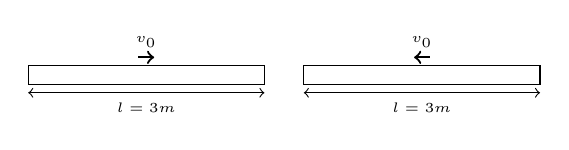
\begin{tikzpicture}
        \draw (0,0) rectangle (3,0.25);
        \draw[<->] (0,-0.1) -- (3,-0.1) node [midway, below] {\tiny $l=3m$};
        \draw[->,thick] (1.4,0.35) -- (1.6,0.35) node [midway, above] {\tiny $v_0$};
        \draw[<->] (3.5,-0.1) -- (6.5,-0.1) node [midway, below] {\tiny $l=3m$};
        \draw[<-,thick] (4.9,0.35) -- (5.1,0.35) node [midway, above] {\tiny $v_0$};
    
        \draw (3.5,0) rectangle (6.5,0.25);
      \end{tikzpicture}
    \end{column}
    \begin{footnotesize}
      \begin{column}{0.49\textwidth}
        $v_0=2.53 \: m/s $; $E= 2\times 10^{11} \: Pa$; $\rho = 7800 \: kg/m^{3}$
      \end{column}
    \end{footnotesize}
  \end{columns}
  \centering
  \begin{tikzpicture}[scale=.675]
\begin{axis}[xlabel=$time \: (s)$,ylabel=$\frac{e}{e_{max}}$,ymajorgrids=true,xmajorgrids=true,legend pos=outer north east,title={Energy plots}]
\addplot[Red,very thick,mark=none,dashed,mark size=2pt] coordinates {(0.0,0.987654320988) (1.2090867954e-05,0.997530864198) (2.41817359079e-05,1.0) (3.62726038619e-05,0.995910493827) (4.83634718158e-05,0.98940007716) (6.04543397698e-05,0.984093484761) (7.25452077237e-05,0.981362538279) (8.46360756777e-05,0.980572573344) (9.67269436317e-05,0.980353499636) (0.000108817811586,0.979737335844) (0.00012090867954,0.97855223305) (0.000132999547494,0.977156270039) (0.000145090415447,0.975958347691) (0.000157181283401,0.97511659562) (0.000169272151355,0.974530084065) (0.000181363019309,0.974005554053) (0.000193453887263,0.97341779498) (0.000205544755217,0.972760977912) (0.000217635623171,0.972101158286) (0.000229726491125,0.971500815494) (0.000241817359079,0.970976328432) (0.000253908227033,0.970503354023) (0.000265999094987,0.970047511625) (0.000278089962941,0.969589945626) (0.000290180830895,0.969132703566) (0.000302271698849,0.968688192138) (0.000314362566803,0.96826592316) (0.000326453434757,0.967866441189) (0.000338544302711,0.96748370195) (0.000350635170665,0.967111035083) (0.000362726038619,0.96674530374) (0.000374816906573,0.9663871534) (0.000386907774527,0.96603867283) (0.000398998642481,0.965701020803) (0.000411089510435,0.9653736209) (0.000423180378389,0.965054863002) (0.000435271246342,0.96474325827) (0.000447362114296,0.964438078134) (0.00045945298225,0.964139187671) (0.000471543850204,0.963846345834) (0.000483634718158,0.963558300848) (0.000495725586112,0.963271635613) (0.000507816454066,0.962978858237) (0.00051990732202,0.962665035247) (0.000531998189974,0.962302555824) (0.000544089057928,0.961844496637) (0.000556179925882,0.961218491107) (0.000568270793836,0.960324692645) (0.00058036166179,0.959042628999) (0.000592452529744,0.95725134199) };
\addplot[Orange,very thick,mark=none,densely dotted,mark size=3pt] coordinates {(0.0,0.987349583462) (1.19687379746e-05,0.997223079297) (2.39374759493e-05,1.0) (3.59062139239e-05,0.996543312249) (4.78749518985e-05,0.991672401699) (5.98436898731e-05,0.988645826067) (7.18124278478e-05,0.98773805255) (8.37811658224e-05,0.987631618227) (9.5749903797e-05,0.987207209533) (0.000107718641772,0.98625862112) (0.000119687379746,0.985162495947) (0.000131656117721,0.984278008796) (0.000143624855696,0.983664883566) (0.00015559359367,0.983176360212) (0.000167562331645,0.982669899583) (0.000179531069619,0.982113551237) (0.000191499807594,0.981554758898) (0.000203468545569,0.981041934115) (0.000215437283543,0.980583060318) (0.000227406021518,0.98015640132) (0.000239374759493,0.979740132791) (0.000251343497467,0.97932838866) (0.000263312235442,0.978927266369) (0.000275280973416,0.978543296202) (0.000287249711391,0.978177057907) (0.000299218449366,0.977824634311) (0.00031118718734,0.977482093196) (0.000323155925315,0.977147995987) (0.00033512466329,0.976822820567) (0.000347093401264,0.976507170495) (0.000359062139239,0.976200756538) (0.000371030877213,0.975902607469) (0.000382999615188,0.97561177268) (0.000394968353163,0.97532772239) (0.000406937091137,0.975050257459) (0.000418905829112,0.974779220922) (0.000430874567087,0.97451432881) (0.000442843305061,0.974255192075) (0.000454812043036,0.974001394871) (0.00046678078101,0.973752448152) (0.000478749518985,0.973507455428) (0.00049071825696,0.973264255861) (0.000502686994934,0.973017591891) (0.000514655732909,0.972755592972) (0.000526624470884,0.972453855054) (0.000538593208858,0.972067038786) (0.000550561946833,0.971519585751) (0.000562530684807,0.970699836135) (0.000574499422782,0.969464605892) (0.000586468160757,0.967662115176) };
\addplot[Duck,thick,mark=*,solid,mark size=2pt] coordinates {(0.0,1.0) (1.19687379746e-05,0.9825) (2.39374759493e-05,0.97517578125) (3.59062139239e-05,0.969031906128) (4.78749518985e-05,0.96380058825) (5.98436898731e-05,0.959171754479) (7.18124278478e-05,0.954982516842) (8.37811658224e-05,0.951129379832) (9.5749903797e-05,0.947543340455) (0.000107718641772,0.944175962079) (0.000119687379746,0.940991760326) (0.000131656117721,0.93796387047) (0.000143624855696,0.935071387013) (0.00015559359367,0.932297671085) (0.000167562331645,0.929629226561) (0.000179531069619,0.927054929147) (0.000191499807594,0.924565482142) (0.000203468545569,0.922153022591) (0.000215437283543,0.91981083008) (0.000227406021518,0.917533107309) (0.000239374759493,0.91531481198) (0.000251343497467,0.913151526055) (0.000263312235442,0.911039352738) (0.000275280973416,0.908974834313) (0.000287249711391,0.906954885898) (0.000299218449366,0.904976741526) (0.00031118718734,0.903037909836) (0.000323155925315,0.901136137378) (0.00033512466329,0.89926937799) (0.000347093401264,0.897435767059) (0.000359062139239,0.895633599746) (0.000371030877213,0.893861312443) (0.000382999615188,0.892117466744) (0.000394968353163,0.890400734736) (0.000406937091137,0.888709882017) (0.000418905829112,0.88704373739) (0.000430874567087,0.88540112132) (0.000442843305061,0.883780678009) (0.000454812043036,0.882180531538) (0.00046678078101,0.880597698856) (0.000478749518985,0.879027284148) (0.00049071825696,0.877461660668) (0.000502686994934,0.875890051367) (0.000514655732909,0.874299006831) (0.000526624470884,0.87267411056) (0.000538593208858,0.871002801233) (0.000550561946833,0.869277656037) (0.000562530684807,0.867499110287) (0.000574499422782,0.865676626234) (0.000586468160757,0.86382779387) };
\addplot[Blue,very thick,mark=none,solid,mark size=3pt] coordinates {(0.0,1.0) (2.41817359079e-05,1.0) (4.83634718158e-05,1.0) (7.25452077237e-05,1.0) (9.67269436317e-05,1.0) (0.00012090867954,1.0) (0.000145090415447,1.0) (0.000169272151355,1.0) (0.000193453887263,1.0) (0.000217635623171,1.0) (0.000241817359079,1.0) (0.000265999094987,1.0) (0.000290180830895,1.0) (0.000314362566803,1.0) (0.000338544302711,1.0) (0.000362726038619,1.0) (0.000386907774527,1.0) (0.000411089510435,1.0) (0.000435271246342,1.0) (0.00045945298225,1.0) (0.000483634718158,1.0) (0.000507816454066,1.0) (0.000531998189974,1.0) (0.000556179925882,1.0) (0.00058036166179,1.0) (0.000604543397698,1.0) };
\addplot[Purple,very thick,mark=+,solid,mark size=3pt] coordinates {(0.0,1.0) (1.19687379746e-05,0.985) (2.39374759493e-05,0.97828125) (3.59062139239e-05,0.972868652344) (4.78749518985e-05,0.968517532349) (5.98436898731e-05,0.964676422477) (7.18124278478e-05,0.961224535313) (8.37811658224e-05,0.95805841396) (9.5749903797e-05,0.955117021818) (0.000107718641772,0.952358340029) (0.000119687379746,0.949751847063) (0.000131656117721,0.947274776455) (0.000143624855696,0.944909512757) (0.00015559359367,0.942642119513) (0.000167562331645,0.940461338934) (0.000179531069619,0.938357922299) (0.000191499807594,0.936324160701) (0.000203468545569,0.934353548006) (0.000215437283543,0.932440533241) (0.000227406021518,0.93058033492) (0.000239374759493,0.928768799379) (0.000251343497467,0.927002291004) (0.000263312235442,0.925277605976) (0.000275280973416,0.923591903662) (0.000287249711391,0.921942651418) (0.000299218449366,0.920327579747) (0.00031118718734,0.918744645509) (0.000323155925315,0.917192001508) (0.00033512466329,0.915667971129) (0.000347093401264,0.91417102706) (0.000359062139239,0.9126997733) (0.000371030877213,0.911252929874) (0.000382999615188,0.909829319753) (0.000394968353163,0.908427857623) (0.000406937091137,0.907047540169) (0.000418905829112,0.905687437658) (0.000430874567087,0.904346686589) (0.000442843305061,0.903024483275) (0.000454812043036,0.901720078186) (0.00046678078101,0.900432770981) (0.000478749518985,0.899161906097) (0.00049071825696,0.897906868838) (0.000502686994934,0.896667081898) (0.000514655732909,0.895442002248) (0.000526624470884,0.894231118352) (0.000538593208858,0.89303394767) (0.000550561946833,0.891850034402) (0.000562530684807,0.890678947462) (0.000574499422782,0.889520278638) (0.000586468160757,0.888373640933) (0.000598436898731,0.887238667044) };
\addplot[Green,thick,mark=x,only marks,mark size=3pt] coordinates {(0.0,1.0) (2.39374759493e-05,1.0) (4.78749518985e-05,1.0) (7.18124278478e-05,1.0) (9.5749903797e-05,1.0) (0.000119687379746,1.0) (0.000143624855696,1.0) (0.000167562331645,1.0) (0.000191499807594,1.0) (0.000215437283543,1.0) (0.000239374759493,1.0) (0.000263312235442,1.0) (0.000287249711391,1.0) (0.00031118718734,1.0) (0.00033512466329,1.0) (0.000359062139239,1.0) (0.000382999615188,1.0) (0.000406937091137,1.0) (0.000430874567087,1.0) (0.000454812043036,1.0) (0.000478749518985,1.0) (0.000502686994934,1.0) (0.000526624470884,1.0) (0.000550561946833,1.0) (0.000574499422782,1.0) (0.000598436898731,1.0) };
\legend{mpm-flip 1ppc -- CFL=0.5,mpm-flip 2ppc -- CFL=0.5,mpm-pic 2ppc -- CFL=0.5,dgmpm 1ppc -- CFL=1,dgmpm 2ppc -- CFL=0.5,dgmpm 2ppc (RK2) -- CFL=1}
\end{axis}
\end{tikzpicture}
%%% Local Variables:
%%% mode: latex
%%% TeX-master: "../../presentation"
%%% End:

  \footnoteCite{Wang}
\end{frame}

\begin{frame}{Riemann problem in a one-dimensional elastic-plastic medium \cite{Thomas_EP}}
  \vskip 5pt
  \begin{columns}
    \begin{column}{0.49\textwidth}
      Plane wave state: $\tens{\eps}=\eps \vect{e}_1 \otimes \vect{e}_1$ % \sigma_{22},\sigma_{33}\neq 0
    \end{column}
    \begin{footnotesize}
      \begin{column}{0.49\textwidth}
        Isotropic linear hardening of modulus $C=10^9 \:Pa$ \\
        $v_0$ leading to plastic flow \\
        %% EP or Elastic Riemann solver coupled to a radial return algorithm \cite{Simo}
      \end{column}
    \end{footnotesize}
  \end{columns}
  \centering
  \begin{tikzpicture}[scale=.6]
\begin{groupplot}[group style={group size=2 by 2,
ylabels at=edge left, yticklabels at=edge left,horizontal sep=2.ex,
vertical sep=4ex,xticklabels at=edge bottom,xlabels at=edge bottom},
ymajorgrids=true,xmajorgrids=true,enlargelimits=0,xmin=0.,xmax=6.,xlabel=$x (m)$,
axis on top,scale only axis,width=0.48\linewidth,legend pos=outer north east
]
\nextgroupplot[title={Incident waves -- Stress},ymin=-1.35e9,ymax=56579516.10614197,]
\addplot[Red,dashed,mark=none,very thick,mark size=3pt,mark repeat=2] coordinates{(0.0,-8433215.03790355) (0.12244897959183673,-31379937.150059074) (0.24489795918367346,-73325965.87671247) (0.36734693877551017,-147815909.35881704) (0.4897959183673469,-264501011.32373637) (0.6122448979591837,-419797360.6339785) (0.7346938775510203,-586994803.1537646) (0.8571428571428571,-715242874.2277462) (0.9795918367346939,-804731796.1198385) (1.1020408163265305,-919403784.9173691) (1.2244897959183674,-1063504114.033879) (1.346938775510204,-1209904754.949398) (1.4693877551020407,-1304654513.0867395) (1.5918367346938775,-1291382612.5749428) (1.7142857142857142,-1218226204.6353252) (1.836734693877551,-1185455835.0777807) (1.9591836734693877,-1232745182.470082) (2.0816326530612246,-1261396271.0817113) (2.204081632653061,-1270103667.4391637) (2.326530612244898,-1227250869.598082) (2.4489795918367347,-1235273389.504192) (2.571428571428571,-1229787858.686364) (2.693877551020408,-1255621316.42765) (2.816326530612245,-1241442333.7811728) (2.9387755102040813,-1239848703.7218106) (3.061224489795918,-1239848703.7218091) (3.183673469387755,-1241442333.781176) (3.306122448979592,-1255621316.4276485) (3.4285714285714284,-1229787858.6863654) (3.5510204081632653,-1235273389.5041904) (3.673469387755102,-1227250869.598084) (3.7959183673469385,-1270103667.439164) (3.9183673469387754,-1261396271.081712) (4.040816326530612,-1232745182.4700806) (4.163265306122449,-1185455835.0777805) (4.285714285714286,-1218226204.6353254) (4.408163265306122,-1291382612.5749435) (4.530612244897959,-1304654513.0867395) (4.653061224489796,-1209904754.9493968) (4.775510204081632,-1063504114.033878) (4.8979591836734695,-919403784.917369) (5.020408163265306,-804731796.1198374) (5.142857142857142,-715242874.2277458) (5.26530612244898,-586994803.1537648) (5.387755102040816,-419797360.63397753) (5.5102040816326525,-264501011.3237358) (5.63265306122449,-147815909.35881624) (5.755102040816326,-73325965.8767119) (5.877551020408163,-31379937.150058918) (6.0,-8433215.037903389) };
\addplot[Blue,solid,mark=+,thick,mark size=3pt,mark repeat=2] coordinates{(0.0,-3.2561158711216654e-07) (0.12244897959183673,-6.54162606232603e-22) (0.24489795918367346,0.0) (0.36734693877551017,3.2561158711216643e-07) (0.4897959183673469,-4.884173806682499e-07) (0.6122448979591837,-710637837.2357953) (0.7346938775510203,-747893724.781927) (0.8571428571428571,-827829409.8631966) (0.9795918367346939,-936780409.853217) (1.1020408163265305,-1054073198.2499647) (1.2244897959183674,-1144128439.1849532) (1.346938775510204,-1207925723.6670742) (1.4693877551020407,-1232372577.7948787) (1.5918367346938775,-1254253728.274747) (1.7142857142857142,-1243570946.3490026) (1.836734693877551,-1268139963.2569304) (1.9591836734693877,-1248035262.8872383) (2.0816326530612246,-1268992337.693115) (2.204081632653061,-1251285653.8729925) (2.326530612244898,-1266352346.5241969) (2.4489795918367347,-1253527311.8706975) (2.571428571428571,-1264419055.233534) (2.693877551020408,-1255474245.0991223) (2.816326530612245,-1261578869.0693417) (2.9387755102040813,-1258168698.6750736) (3.061224489795918,-1258168698.6750731) (3.183673469387755,-1261578869.069342) (3.306122448979592,-1255474245.0991209) (3.4285714285714284,-1264419055.233534) (3.5510204081632653,-1253527311.870696) (3.673469387755102,-1266352346.5241973) (3.7959183673469385,-1251285653.8729923) (3.9183673469387754,-1268992337.6931143) (4.040816326530612,-1248035262.8872375) (4.163265306122449,-1268139963.2569308) (4.285714285714286,-1243570946.3490026) (4.408163265306122,-1254253728.2747467) (4.530612244897959,-1232372577.7948787) (4.653061224489796,-1207925723.6670735) (4.775510204081632,-1144128439.1849532) (4.8979591836734695,-1054073198.2499645) (5.020408163265306,-936780409.853217) (5.142857142857142,-827829409.8631967) (5.26530612244898,-747893724.7819276) (5.387755102040816,-710637837.2357956) (5.5102040816326525,-4.884173806682498e-07) (5.63265306122449,0.0) (5.755102040816326,-4.884173806682498e-07) (5.877551020408163,0.0) (6.0,-4.884173806682498e-07) };
\addplot[Orange,solid,mark=o,very thick,mark size=2pt,mark repeat=2] coordinates{(0.0,0.0) (0.12244897959183673,0.0) (0.24489795918367346,0.0) (0.36734693877551017,0.0) (0.4897959183673469,0.0) (0.6122448979591837,-700099961.461325) (0.7346938775510203,-702215400.6707044) (0.8571428571428571,-720845446.6905135) (0.9795918367346939,-807249777.2239016) (1.1020408163265305,-1021817726.088786) (1.2244897959183674,-1257135415.8766613) (1.346938775510204,-1201909815.2742617) (1.4693877551020407,-1284541316.0967622) (1.5918367346938775,-1197762497.5853782) (1.7142857142857142,-1280230396.1356874) (1.836734693877551,-1230639248.475009) (1.9591836734693877,-1232614670.2907715) (2.0816326530612246,-1296340561.1434355) (2.204081632653061,-1163180742.3691304) (2.326530612244898,-1344085453.2920678) (2.4489795918367347,-1125286993.986051) (2.571428571428571,-1354573027.5700727) (2.693877551020408,-1144440690.6862848) (2.816326530612245,-1331966839.3238678) (2.9387755102040813,-1234245710.8866477) (3.061224489795918,-1234245710.8866642) (3.183673469387755,-1331966839.3238637) (3.306122448979592,-1144440690.6862931) (3.4285714285714284,-1354573027.570076) (3.5510204081632653,-1125286993.9860492) (3.673469387755102,-1344085453.2920709) (3.7959183673469385,-1163180742.369132) (3.9183673469387754,-1296340561.143439) (4.040816326530612,-1232614670.2907667) (4.163265306122449,-1230639248.4750104) (4.285714285714286,-1280230396.1356888) (4.408163265306122,-1197762497.5853772) (4.530612244897959,-1284541316.0967634) (4.653061224489796,-1201909815.2742698) (4.775510204081632,-1257135415.8766532) (4.8979591836734695,-1021817726.0887933) (5.020408163265306,-807249777.2238963) (5.142857142857142,-720845446.6905184) (5.26530612244898,-702215400.6706979) (5.387755102040816,-700099961.4613259) (5.5102040816326525,0.0) (5.63265306122449,0.0) (5.755102040816326,0.0) (5.877551020408163,0.0) (6.0,0.0) };
\addplot[Purple,solid,mark=x,thick,mark size=3pt,mark repeat=2] coordinates{(0.0,0.0) (0.12244897959183673,0.0) (0.24489795918367346,0.0) (0.36734693877551017,0.0) (0.4897959183673469,0.0) (0.6122448979591837,-700149009.8511133) (0.7346938775510203,-702792255.866507) (0.8571428571428571,-725326867.326901) (0.9795918367346939,-850156660.8530495) (1.1020408163265305,-1109984935.9712873) (1.2244897959183674,-1250258832.4370122) (1.346938775510204,-1260471082.9558206) (1.4693877551020407,-1260981625.9873586) (1.5918367346938775,-1261003693.8957453) (1.7142857142857142,-1261004546.9659622) (1.836734693877551,-1261004575.4299965) (1.9591836734693877,-1261004576.2405941) (2.0816326530612246,-1261004576.260158) (2.204081632653061,-1261004576.2605524) (2.326530612244898,-1261004576.260559) (2.4489795918367347,-1261004576.260559) (2.571428571428571,-1261004576.260559) (2.693877551020408,-1261004576.260559) (2.816326530612245,-1261004576.2605588) (2.9387755102040813,-1261004576.2605588) (3.061224489795918,-1261004576.260559) (3.183673469387755,-1261004576.2605588) (3.306122448979592,-1261004576.2605588) (3.4285714285714284,-1261004576.2605588) (3.5510204081632653,-1261004576.2605588) (3.673469387755102,-1261004576.2605588) (3.7959183673469385,-1261004576.260553) (3.9183673469387754,-1261004576.2601585) (4.040816326530612,-1261004576.2405944) (4.163265306122449,-1261004575.4299967) (4.285714285714286,-1261004546.9659626) (4.408163265306122,-1261003693.895745) (4.530612244897959,-1260981625.987358) (4.653061224489796,-1260471082.955823) (4.775510204081632,-1250258832.4370096) (4.8979591836734695,-1109984935.971287) (5.020408163265306,-850156660.8530501) (5.142857142857142,-725326867.326901) (5.26530612244898,-702792255.866507) (5.387755102040816,-700149009.8511133) (5.5102040816326525,0.0) (5.63265306122449,0.0) (5.755102040816326,0.0) (5.877551020408163,0.0) (6.0,0.0) };
\addplot[black,solid,mark=none,thin,mark size=3pt,mark repeat=2] coordinates{(0.0,-0.0) (0.12244897959183673,-0.0) (0.24489795918367346,-0.0) (0.36734693877551017,-0.0) (0.4897959183673469,-0.0) (0.6122448979591837,-700000000.0) (0.7346938775510203,-700000000.0) (0.8571428571428571,-700000000.0) (0.9795918367346939,-700000000.0) (1.1020408163265305,-1261004576.260559) (1.2244897959183674,-1261004576.260559) (1.346938775510204,-1261004576.260559) (1.4693877551020407,-1261004576.260559) (1.5918367346938775,-1261004576.260559) (1.7142857142857142,-1261004576.260559) (1.836734693877551,-1261004576.260559) (1.9591836734693877,-1261004576.260559) (2.0816326530612246,-1261004576.260559) (2.204081632653061,-1261004576.260559) (2.326530612244898,-1261004576.260559) (2.4489795918367347,-1261004576.260559) (2.571428571428571,-1261004576.260559) (2.693877551020408,-1261004576.260559) (2.816326530612245,-1261004576.260559) (2.9387755102040813,-1261004576.260559) (3.061224489795918,-1261004576.260559) (3.183673469387755,-1261004576.260559) (3.306122448979592,-1261004576.260559) (3.4285714285714284,-1261004576.260559) (3.5510204081632653,-1261004576.260559) (3.673469387755102,-1261004576.260559) (3.7959183673469385,-1261004576.260559) (3.9183673469387754,-1261004576.260559) (4.040816326530612,-1261004576.260559) (4.163265306122449,-1261004576.260559) (4.285714285714286,-1261004576.260559) (4.408163265306122,-1261004576.260559) (4.530612244897959,-1261004576.260559) (4.653061224489796,-1261004576.260559) (4.775510204081632,-1261004576.260559) (4.8979591836734695,-1261004576.260559) (5.020408163265306,-700000000.0) (5.142857142857142,-700000000.0) (5.26530612244898,-700000000.0) (5.387755102040816,-700000000.0) (5.5102040816326525,-0.0) (5.63265306122449,-0.0) (5.755102040816326,-0.0) (5.877551020408163,-0.0) (6.0,-0.0) };
\addlegendentry{mpm}
\addlegendentry{dgmpm}
\addlegendentry{fem}
\addlegendentry{fvm (SB)}
\addlegendentry{exact}

\end{groupplot}
\end{tikzpicture}
%%% Local Variables:
%%% mode: latex
%%% TeX-master: "../../presentation"
%%% End:

  \footnoteCite{Thomas_EP}
\end{frame}

\begin{frame}{Riemann problem in a one-dimensional elastic-plastic medium \cite{Thomas_EP}}
  \vskip 5pt
  \begin{columns}
    \begin{column}{0.49\textwidth}
      Plane wave state: $\tens{\eps}=\eps \vect{e}_1 \otimes \vect{e}_1$ % \sigma_{22},\sigma_{33}\neq 0
    \end{column}
    \begin{footnotesize}
      \begin{column}{0.49\textwidth}
        Isotropic linear hardening of modulus $C=10^9 \:Pa$ \\
        $v_0$ leading to plastic flow \\
        %% EP or Elastic Riemann solver coupled to a radial return algorithm \cite{Simo}
      \end{column}
    \end{footnotesize}
  \end{columns}
    \centering
    \begin{tikzpicture}[scale=.6]
\begin{groupplot}[group style={group size=2 by 2,
ylabels at=edge left, yticklabels at=edge left,horizontal sep=2.ex,
vertical sep=4ex,xticklabels at=edge bottom,xlabels at=edge bottom},
ymajorgrids=true,xmajorgrids=true,enlargelimits=0,xmin=0.,xmax=6.,xlabel=$x (m)$,
axis on top,scale only axis,width=0.48\linewidth,legend pos=outer north east
]

\nextgroupplot[title={Incident waves -- Plastic strain},ymin=-0.0034,ymax=0.0,xlabel=$x \:(m)$,ylabel=$\eps^p$]
\addplot[Red,dashed,mark=none,very thick,mark size=3pt,mark repeat=2] coordinates{(0.0,0.0) (0.12244897959183673,0.0) (0.24489795918367346,0.0) (0.36734693877551017,0.0) (0.4897959183673469,0.0) (0.6122448979591837,0.0) (0.7346938775510203,0.0) (0.8571428571428571,-5.5177825258810104e-05) (0.9795918367346939,-0.0003791196239632164) (1.1020408163265305,-0.0007942218458547296) (1.2244897959183674,-0.0013158519965027296) (1.346938775510204,-0.0018458090676901286) (1.4693877551020407,-0.002188794617508559) (1.5918367346938775,-0.002229697455331896) (1.7142857142857142,-0.002258121963594508) (1.836734693877551,-0.002271799079674154) (1.9591836734693877,-0.002320613632318322) (2.0816326530612246,-0.002313868472160546) (2.204081632653061,-0.0024020122032007017) (2.326530612244898,-0.0023588630990294623) (2.4489795918367347,-0.0025433455597807667) (2.571428571428571,-0.002385435935351422) (2.693877551020408,-0.0027693350417516906) (2.816326530612245,-0.0024065265204776445) (2.9387755102040813,-0.0032250612006492966) (3.061224489795918,-0.0032250612006492524) (3.183673469387755,-0.002406526520477666) (3.306122448979592,-0.0027693350417516823) (3.4285714285714284,-0.0023854359353514295) (3.5510204081632653,-0.0025433455597807628) (3.673469387755102,-0.002358863099029464) (3.7959183673469385,-0.0024020122032006983) (3.9183673469387754,-0.0023138684721605448) (4.040816326530612,-0.002320613632318319) (4.163265306122449,-0.0022717990796741546) (4.285714285714286,-0.0022581219635945077) (4.408163265306122,-0.0022296974553318956) (4.530612244897959,-0.0021887946175085595) (4.653061224489796,-0.001845809067690125) (4.775510204081632,-0.0013158519965027254) (4.8979591836734695,-0.0007942218458547295) (5.020408163265306,-0.0003791196239632123) (5.142857142857142,-5.5177825258808404e-05) (5.26530612244898,0.0) (5.387755102040816,0.0) (5.5102040816326525,0.0) (5.63265306122449,0.0) (5.755102040816326,0.0) (5.877551020408163,0.0) (6.0,0.0) };
\addplot[Blue,solid,mark=+,thick,mark size=3pt,mark repeat=2] coordinates{(0.0,0.0) (0.12244897959183673,0.0) (0.24489795918367346,0.0) (0.36734693877551017,0.0) (0.4897959183673469,0.0) (0.6122448979591837,-3.850800809337606e-05) (0.7346938775510203,-0.00017337094943683953) (0.8571428571428571,-0.00046273089543238553) (0.9795918367346939,-0.000857123655577256) (1.1020408163265305,-0.0012817129348415013) (1.2244897959183674,-0.0016077047572306) (1.346938775510204,-0.0018386451535459692) (1.4693877551020407,-0.0019271405531036338) (1.5918367346938775,-0.002006348337646142) (1.7142857142857142,-0.002018045326373221) (1.836734693877551,-0.002056615251608797) (1.9591836734693877,-0.0020613216365693464) (2.0816326530612246,-0.002064203896841495) (2.204081632653061,-0.0020644266901542695) (2.326530612244898,-0.0020621094945296272) (2.4489795918367347,-0.002062767607181189) (2.571428571428571,-0.002061489252343496) (2.693877551020408,-0.0020573197208032658) (2.816326530612245,-0.0020502799029179) (2.9387755102040813,-0.0020377776694292327) (3.061224489795918,-0.0020377776694292327) (3.183673469387755,-0.002050279902917899) (3.306122448979592,-0.002057319720803265) (3.4285714285714284,-0.0020614892523434956) (3.5510204081632653,-0.0020627676071811878) (3.673469387755102,-0.0020621094945296285) (3.7959183673469385,-0.0020644266901542695) (3.9183673469387754,-0.0020642038968414953) (4.040816326530612,-0.0020613216365693477) (4.163265306122449,-0.002056615251608799) (4.285714285714286,-0.0020180453263732205) (4.408163265306122,-0.0020063483376461405) (4.530612244897959,-0.0019271405531036334) (4.653061224489796,-0.0018386451535459673) (4.775510204081632,-0.0016077047572305996) (4.8979591836734695,-0.0012817129348415002) (5.020408163265306,-0.0008571236555772557) (5.142857142857142,-0.000462730895432386) (5.26530612244898,-0.0001733709494368422) (5.387755102040816,-3.850800809337776e-05) (5.5102040816326525,0.0) (5.63265306122449,0.0) (5.755102040816326,0.0) (5.877551020408163,0.0) (6.0,0.0) };
\addplot[Orange,solid,mark=o,very thick,mark size=2pt,mark repeat=2] coordinates{(0.0,0.0) (0.12244897959183673,0.0) (0.24489795918367346,0.0) (0.36734693877551017,0.0) (0.4897959183673469,0.0) (0.6122448979591837,-3.6185144371068533e-07) (0.7346938775510203,-8.019549939201378e-06) (0.8571428571428571,-7.545863055389513e-05) (0.9795918367346939,-0.00038823448768833166) (1.1020408163265305,-0.0011649510446652884) (1.2244897959183674,-0.0020167797859788647) (1.346938775510204,-0.002107399619958115) (1.4693877551020407,-0.002131770374563102) (1.5918367346938775,-0.0021403574192086572) (1.7142857142857142,-0.0021224712498380525) (1.836734693877551,-0.0021223153729543927) (1.9591836734693877,-0.002051517588290279) (2.0816326530612246,-0.00215869886386764) (2.204081632653061,-0.00229323761080671) (2.326530612244898,-0.002383730340592019) (2.4489795918367347,-0.002422023782426279) (2.571428571428571,-0.0024301527006305407) (2.693877551020408,-0.0023776240406298606) (2.816326530612245,-0.0022924966391795762) (2.9387755102040813,-0.002209718054457858) (3.061224489795918,-0.002209718054457853) (3.183673469387755,-0.00229249663917957) (3.306122448979592,-0.002377624040629834) (3.4285714285714284,-0.0024301527006305133) (3.5510204081632653,-0.0024220237824262893) (3.673469387755102,-0.0023837303405920274) (3.7959183673469385,-0.0022932376108067225) (3.9183673469387754,-0.002158698863867652) (4.040816326530612,-0.0020515175882902612) (4.163265306122449,-0.00212231537295439) (4.285714285714286,-0.002122471249838043) (4.408163265306122,-0.002140357419208655) (4.530612244897959,-0.0021317703745630944) (4.653061224489796,-0.0021073996199581038) (4.775510204081632,-0.002016779785978835) (4.8979591836734695,-0.0011649510446653149) (5.020408163265306,-0.00038823448768831226) (5.142857142857142,-7.54586305539126e-05) (5.26530612244898,-8.019549939178096e-06) (5.387755102040816,-3.6185144371335306e-07) (5.5102040816326525,0.0) (5.63265306122449,0.0) (5.755102040816326,0.0) (5.877551020408163,0.0) (6.0,0.0) };
\addplot[Purple,solid,mark=x,thick,mark size=3pt,mark repeat=2] coordinates{(0.0,0.0) (0.12244897959183673,0.0) (0.24489795918367346,0.0) (0.36734693877551017,0.0) (0.4897959183673469,0.0) (0.6122448979591837,-5.394021759754931e-07) (0.7346938775510203,-1.010771354391672e-05) (0.8571428571428571,-9.168096769918878e-05) (0.9795918367346939,-0.0005435535234499527) (1.1020408163265305,-0.0014841083655069223) (1.2244897959183674,-0.001991887176242578) (1.346938775510204,-0.002028854598935097) (1.4693877551020407,-0.0020307027185062754) (1.5918367346938775,-0.002030782602337539) (1.7142857142857142,-0.0020307856903745234) (1.836734693877551,-0.002030785793411752) (1.9591836734693877,-0.002030785796346042) (2.0816326530612246,-0.002030785796416862) (2.204081632653061,-0.002030785796418289) (2.326530612244898,-0.0020307857964183135) (2.4489795918367347,-0.0020307857964183135) (2.571428571428571,-0.0020307857964183135) (2.693877551020408,-0.0020307857964183135) (2.816326530612245,-0.0020307857964183135) (2.9387755102040813,-0.0020307857964183135) (3.061224489795918,-0.0020307857964183135) (3.183673469387755,-0.0020307857964183135) (3.306122448979592,-0.0020307857964183126) (3.4285714285714284,-0.0020307857964183135) (3.5510204081632653,-0.0020307857964183126) (3.673469387755102,-0.0020307857964183126) (3.7959183673469385,-0.002030785796418291) (3.9183673469387754,-0.0020307857964168632) (4.040816326530612,-0.0020307857963460427) (4.163265306122449,-0.0020307857934117523) (4.285714285714286,-0.002030785690374525) (4.408163265306122,-0.0020307826023375384) (4.530612244897959,-0.0020307027185062733) (4.653061224489796,-0.002028854598935106) (4.775510204081632,-0.0019918871762425686) (4.8979591836734695,-0.0014841083655069208) (5.020408163265306,-0.0005435535234499549) (5.142857142857142,-9.168096769918878e-05) (5.26530612244898,-1.010771354391672e-05) (5.387755102040816,-5.394021759754931e-07) (5.5102040816326525,0.0) (5.63265306122449,0.0) (5.755102040816326,0.0) (5.877551020408163,0.0) (6.0,0.0) };
\addplot[black,solid,mark=none,thin,mark size=3pt,mark repeat=2] coordinates{(0.0,-0.0) (0.12244897959183673,-0.0) (0.24489795918367346,-0.0) (0.36734693877551017,-0.0) (0.4897959183673469,-0.0) (0.6122448979591837,-0.0) (0.7346938775510203,-0.0) (0.8571428571428571,-0.0) (0.9795918367346939,-0.0) (1.1020408163265305,-0.002030785796418313) (1.2244897959183674,-0.002030785796418313) (1.346938775510204,-0.002030785796418313) (1.4693877551020407,-0.002030785796418313) (1.5918367346938775,-0.002030785796418313) (1.7142857142857142,-0.002030785796418313) (1.836734693877551,-0.002030785796418313) (1.9591836734693877,-0.002030785796418313) (2.0816326530612246,-0.002030785796418313) (2.204081632653061,-0.002030785796418313) (2.326530612244898,-0.002030785796418313) (2.4489795918367347,-0.002030785796418313) (2.571428571428571,-0.002030785796418313) (2.693877551020408,-0.002030785796418313) (2.816326530612245,-0.002030785796418313) (2.9387755102040813,-0.002030785796418313) (3.061224489795918,-0.002030785796418313) (3.183673469387755,-0.002030785796418313) (3.306122448979592,-0.002030785796418313) (3.4285714285714284,-0.002030785796418313) (3.5510204081632653,-0.002030785796418313) (3.673469387755102,-0.002030785796418313) (3.7959183673469385,-0.002030785796418313) (3.9183673469387754,-0.002030785796418313) (4.040816326530612,-0.002030785796418313) (4.163265306122449,-0.002030785796418313) (4.285714285714286,-0.002030785796418313) (4.408163265306122,-0.002030785796418313) (4.530612244897959,-0.002030785796418313) (4.653061224489796,-0.002030785796418313) (4.775510204081632,-0.002030785796418313) (4.8979591836734695,-0.002030785796418313) (5.020408163265306,-0.0) (5.142857142857142,-0.0) (5.26530612244898,-0.0) (5.387755102040816,-0.0) (5.5102040816326525,-0.0) (5.63265306122449,-0.0) (5.755102040816326,-0.0) (5.877551020408163,-0.0) (6.0,-0.0) };
\addlegendentry{mpm}
\addlegendentry{dgmpm}
\addlegendentry{fem}
\addlegendentry{fvm (SB)}
\addlegendentry{exact}

\end{groupplot}
\end{tikzpicture}
%%% Local Variables:
%%% mode: latex
%%% TeX-master: "../../presentation"
%%% End:

    \footnoteCite{Thomas_EP}
\end{frame}

% \begin{frame}{\href{section4/animation/elasticity_stress/video.mp4}{Plane strain elasticity}}
%   \begin{overprint}
%     \onslide<1>
%     \vspace{-1.cm}
%     \begin{columns}
%       \begin{column}{0.42\linewidth}
%         \input{section4/pgfFigures/2d_square}
%       \end{column}

%       \begin{column}{0.6\linewidth}
%         \vspace{1.5cm}
%         \centering
%         \phantom{\begin{tikzpicture}
  \begin{groupplot}[group style={group size=2 by 1,
ylabels at=edge left, yticklabels at=edge left,horizontal sep=1.5ex,
xticklabels at=edge bottom,xlabels at=edge bottom},
ymajorgrids=true,xmajorgrids=true,xlabel=$x \: (m)$,
axis on top,scale only axis,width=0.43\linewidth, every x tick scale label/.style={at={(xticklabel* cs:1.05,0.75cm)},anchor=near yticklabel},ymin=-0.5e6,ymax=.5e9,xmin=0,xmax=3]
\nextgroupplot[ylabel=$\sigma_{11}\: (Pa)$,title={$t=2.5 \times 10^{-4} \: s$},every y tick scale label/.style={at={(-0.,1.1)}}]
\addplot[Red,very thick,no markers] table[x=Points:0,y=S11] {section4/csvFiles/2delast_fem_115.csv};

\addplot[Blue,very thick,mark=+,only marks,mark size=3pt] table[x=Points:0,y=stress_11] {section4/csvFiles/2delast_ctu1ppc_115.csv};
\addplot[Purple,very thick,mark=asterisk,only marks,mark size=2pt] table[x=Points:0,y=stress_11] {section4/csvFiles/2delast_ctu4ppc_115.csv};
\addplot[Orange,very thick,mark=x,only marks,mark size=3pt] table[x=Points:0,y=mpm_S11] {section4/csvFiles/2delast_mpm_115.csv};

\nextgroupplot[legend style={at={($(0.22,-0.3)+(1.cm,0cm)$)},legend columns=2},xlabel=$x (m)$,title={$t=1.0 \times 10^{-3} \: s$},ytick scale label code/.code={}]
\addplot[Red,very thick,no markers] table[x=Points:0,y=S11] {section4/csvFiles/2delast_fem_338.csv};
\addplot[Blue,very thick,mark=+,only marks,mark size=3pt] table[x=Points:0,y=stress_11] {section4/csvFiles/2delast_ctu1ppc_338.csv};
\addplot[Purple,very thick,mark=asterisk,only marks,mark size=2pt] table[x=Points:0,y=stress_11] {section4/csvFiles/2delast_ctu4ppc_338.csv};
\addplot[Orange,very thick,mark=x,only marks,mark size=3pt] table[x=Points:0,y=mpm_S11] {section4/csvFiles/2delast_mpm_338.csv};
\addlegendentry{fem}
\addlegendentry{ctu 1ppc}
\addlegendentry{ctu 4ppc}
\addlegendentry{mpm}
   
  \end{groupplot}
\end{tikzpicture}


%%% Local Variables:
%%% mode: latex
%%% TeX-master: "../../aRenaud"
%%% End:




































%%% Local Variables:
%%% mode: latex
%%% TeX-master: "../../mainManuscript"
%%% End:
}
%       \end{column}
      
%     \end{columns}
%     \onslide<2>
%     \vspace{-1.cm}
%     \begin{columns}
%       \begin{column}{0.4\linewidth}
%         \movie[height=.7\paperheight,width=1.\linewidth,showcontrols,loop,poster,autostart]{%\input{section4/pgfFigures/2d_square}
%         }{section4/animation/elasticity_stress/out.mp4}
%       \end{column}

%       \begin{column}{0.6\linewidth}
%         \vspace{1.5cm}
%         \centering
%         \begin{tikzpicture}
  \begin{groupplot}[group style={group size=2 by 1,
ylabels at=edge left, yticklabels at=edge left,horizontal sep=1.5ex,
xticklabels at=edge bottom,xlabels at=edge bottom},
ymajorgrids=true,xmajorgrids=true,xlabel=$x \: (m)$,
axis on top,scale only axis,width=0.43\linewidth, every x tick scale label/.style={at={(xticklabel* cs:1.05,0.75cm)},anchor=near yticklabel},ymin=-0.5e6,ymax=.5e9,xmin=0,xmax=3]
\nextgroupplot[ylabel=$\sigma_{11}\: (Pa)$,title={$t=2.5 \times 10^{-4} \: s$},every y tick scale label/.style={at={(-0.,1.1)}}]
\addplot[Red,very thick,no markers] table[x=Points:0,y=S11] {section4/csvFiles/2delast_fem_115.csv};

\addplot[Blue,very thick,mark=+,only marks,mark size=3pt] table[x=Points:0,y=stress_11] {section4/csvFiles/2delast_ctu1ppc_115.csv};
\addplot[Purple,very thick,mark=asterisk,only marks,mark size=2pt] table[x=Points:0,y=stress_11] {section4/csvFiles/2delast_ctu4ppc_115.csv};
\addplot[Orange,very thick,mark=x,only marks,mark size=3pt] table[x=Points:0,y=mpm_S11] {section4/csvFiles/2delast_mpm_115.csv};

\nextgroupplot[legend style={at={($(0.22,-0.3)+(1.cm,0cm)$)},legend columns=2},xlabel=$x (m)$,title={$t=1.0 \times 10^{-3} \: s$},ytick scale label code/.code={}]
\addplot[Red,very thick,no markers] table[x=Points:0,y=S11] {section4/csvFiles/2delast_fem_338.csv};
\addplot[Blue,very thick,mark=+,only marks,mark size=3pt] table[x=Points:0,y=stress_11] {section4/csvFiles/2delast_ctu1ppc_338.csv};
\addplot[Purple,very thick,mark=asterisk,only marks,mark size=2pt] table[x=Points:0,y=stress_11] {section4/csvFiles/2delast_ctu4ppc_338.csv};
\addplot[Orange,very thick,mark=x,only marks,mark size=3pt] table[x=Points:0,y=mpm_S11] {section4/csvFiles/2delast_mpm_338.csv};
\addlegendentry{fem}
\addlegendentry{ctu 1ppc}
\addlegendentry{ctu 4ppc}
\addlegendentry{mpm}
   
  \end{groupplot}
\end{tikzpicture}


%%% Local Variables:
%%% mode: latex
%%% TeX-master: "../../aRenaud"
%%% End:




































%%% Local Variables:
%%% mode: latex
%%% TeX-master: "../../mainManuscript"
%%% End:

%       \end{column}
%     \end{columns}
%   \end{overprint}
% \end{frame}


\begin{frame}{\href{section4/animation/elastoplasticity_p/video.mp4}{Plane strain elastoplasticity}}
  Parler de Castem -- ecrouissage
  \begin{overprint}
    \onslide<1>
    \begin{block}
      \centering
      \input{section4/pgfFigures/2d_square}
    \end{block}
    \onslide<2>
    \vspace{0.25cm}
    \centering
    \movie[height=.69\paperheight,width=.49\linewidth,showcontrols,loop,poster,autostart]{}{section4/animation/elastoplasticity_p/video.mp4}
    \onslide<3>
    \vspace{0.05cm}
    \centering
    \begin{tikzpicture}[scale=0.49]
  \begin{groupplot}[group style={group size=1 by 2,
ylabels at=edge left, yticklabels at=edge left,horizontal sep=3.ex,vertical sep=4.ex,
xticklabels at=edge bottom,xlabels at=edge bottom},
ymajorgrids=true,xmajorgrids=true,
axis on top,scale only axis, every x tick scale label/.style={at={(xticklabel* cs:1.05,0.75cm)},anchor=near yticklabel}]
\nextgroupplot[ylabel=\normalsize $\sigma_{11}$ (Pa)]
\addplot[Red,very thick,no markers] table[x=Points:0,y=S11] {appendix/csvFiles/2dEP_fem_115.csv};
\addplot[Blue,very thick,mark=+,only marks,mark size=3pt] table[x=Points:0,y=stress_11] {appendix/csvFiles/2dEP_ctu1ppc_115.csv};
\addplot[Purple,very thick,mark=square,only marks] table[x=Points:0,y=stress_11] {appendix/csvFiles/2dEP_ctu4ppc_115.csv};
\addplot[Orange,very thick,mark=x,only marks,mark size=3pt] table[x=Points:0,y= mpm_S11] {appendix/csvFiles/2dEP_mpm_115.csv};

% \nextgroupplot[title={(b) $t=1.0 \times 10^{-3} \: s$},ymin=-0.5e6,ymax=1.5e9]
% \addplot[Red,very thick,no markers] table[x=Points:0,y=S11] {appendix/csvFiles/2dEP_fem_338.csv};
% \addplot[Blue,very thick,mark=+,only marks,mark size=3pt] table[x=Points:0,y=stress_11] {appendix/csvFiles/2dEP_ctu1ppc_338.csv};
% \addplot[Purple,very thick,mark=square,only marks] table[x=Points:0,y=stress_11] {appendix/csvFiles/2dEP_ctu4ppc_338.csv};
% \addplot[Orange,very thick,mark=x,only marks,mark size=3pt] table[x=Points:0,y= mpm_S11] {appendix/csvFiles/2dEP_mpm_338.csv};

\nextgroupplot[%legend style={at={($(0.12,-0.35)+(5cm,5cm)$)},legend columns=1}
legend pos={north east},
,ylabel=\normalsize $\eps^p_{11}$,xlabel=\normalsize $x$ (m)]
\addplot[Red,very thick,no markers] table[x=Points:0,y=EP11] {appendix/csvFiles/2dEP_fem_115.csv};
\addplot[Blue,very thick,mark=+,only marks,mark size=3pt] table[x=Points:0,y=epsp_11] {appendix/csvFiles/2dEP_ctu1ppc_115.csv};
\addplot[Purple,very thick,mark=square,only marks] table[x=Points:0,y=epsp_11] {appendix/csvFiles/2dEP_ctu4ppc_115.csv};
\addplot[Orange,very thick,mark=x,only marks,mark size=3pt] table[x=Points:0,y= mpm_epsp11] {appendix/csvFiles/2dEP_mpm_115.csv};

% \nextgroupplot[legend style={at={($(0.12,-0.35)+(0.9cm,1cm)$)},legend columns=2},xlabel=$x (m)$,ymin=-0.1e-3,ymax=6.75e-3]
% \addplot[Red,very thick,no markers] table[x=Points:0,y=EP11] {appendix/csvFiles/2dEP_fem_338.csv};
% \addplot[Blue,very thick,mark=+,only marks,mark size=3pt] table[x=Points:0,y=epsp_11] {appendix/csvFiles/2dEP_ctu1ppc_338.csv};
% \addplot[Purple,very thick,mark=square,only marks] table[x=Points:0,y=epsp_11] {appendix/csvFiles/2dEP_ctu4ppc_338.csv};
% \addplot[Orange,very thick,mark=x,only marks,mark size=3pt] table[x=Points:0,y= mpm_epsp11] {appendix/csvFiles/2dEP_mpm_338.csv};
\addlegendentry{fem}
\addlegendentry{ctu 1ppc}
\addlegendentry{ctu 4ppc}
\addlegendentry{mpm}
   
  \end{groupplot}
\end{tikzpicture}


%%% Local Variables:
%%% mode: latex
%%% TeX-master: "../../presentation"
%%% End:




































%%% Local Variables:
%%% mode: latex
%%% TeX-master: "../../presentation"
%%% End:

  \end{overprint}

\end{frame}


%%% Local Variables:
%%% mode: latex
%%% TeX-master: "../presentation"
%%% End: